\documentclass[a4paper,12pt,twoside]{memoir}

% Castellano
\usepackage[spanish,es-tabla]{babel}
\selectlanguage{spanish}
\usepackage[utf8]{inputenc}
\usepackage[T1]{fontenc}
\usepackage{lmodern} % scalable font
\usepackage{microtype}
\usepackage{placeins}
\usepackage{booktabs}
\usepackage[smartEllipses]{markdown}
\usepackage{pdfpages}
\usepackage[hashEnumerators,smartEllipses]{markdown}
\RequirePackage{booktabs}
\RequirePackage[table]{xcolor}
\RequirePackage{xtab}
\RequirePackage{multirow}
\usepackage{longtable}

\def\checkmark{\tikz\fill[scale=0.4](0,.35) -- (.25,0) -- (1,.7) -- (.25,.15) -- cycle;} 
% Links
\PassOptionsToPackage{hyphens}{url}\usepackage[colorlinks]{hyperref}
\hypersetup{
	allcolors = {red}
}

% Ecuaciones
\usepackage{amsmath}

% Rutas de fichero / paquete
\newcommand{\ruta}[1]{{\sffamily #1}}

\usepackage{tikz}
\def\checkmark{\tikz\fill[scale=0.4](0,.35) -- (.25,0) -- (1,.7) -- (.25,.15) -- cycle;} 

% Párrafos
\nonzeroparskip

% Huérfanas y viudas
\widowpenalty100000
\clubpenalty100000

% Evitar solapes en el header
\nouppercaseheads

% Imagenes
\usepackage{graphicx}
\newcommand{\imagen}[2]{
	\begin{figure}[!h]
		\centering
		\includegraphics[width=0.9\textwidth]{#1}
		\caption{#2}\label{fig:#1}
	\end{figure}
	\FloatBarrier
}

\newcommand{\imagenflotante}[2]{
	\begin{figure}%[!h]
		\centering
		\includegraphics[width=0.9\textwidth]{#1}
		\caption{#2}\label{fig:#1}
	\end{figure}
}



% El comando \figura nos permite insertar figuras comodamente, y utilizando
% siempre el mismo formato. Los parametros son:
% 1 -> Porcentaje del ancho de página que ocupará la figura (de 0 a 1)
% 2 --> Fichero de la imagen
% 3 --> Texto a pie de imagen
% 4 --> Etiqueta (label) para referencias
% 5 --> Opciones que queramos pasarle al \includegraphics
% 6 --> Opciones de posicionamiento a pasarle a \begin{figure}
\newcommand{\figuraConPosicion}[6]{%
  \setlength{\anchoFloat}{#1\textwidth}%
  \addtolength{\anchoFloat}{-4\fboxsep}%
  \setlength{\anchoFigura}{\anchoFloat}%
  \begin{figure}[#6]
    \begin{center}%
      \Ovalbox{%
        \begin{minipage}{\anchoFloat}%
          \begin{center}%
            \includegraphics[width=\anchoFigura,#5]{#2}%
            \caption{#3}%
            \label{#4}%
          \end{center}%
        \end{minipage}
      }%
    \end{center}%
  \end{figure}%
}

%
% Comando para incluir imágenes en formato apaisado (sin marco).
\newcommand{\figuraApaisadaSinMarco}[5]{%
  \begin{figure}%
    \begin{center}%
    \includegraphics[angle=90,height=#1\textheight,#5]{#2}%
    \caption{#3}%
    \label{#4}%
    \end{center}%
  \end{figure}%
}
% Para las tablas
\newcommand{\otoprule}{\midrule [\heavyrulewidth]}
%
% Nuevo comando para tablas pequeñas (menos de una página).
\newcommand{\tablaSmall}[5]{%
 \begin{table}
  \begin{center}
   \rowcolors {2}{gray!35}{}
   \begin{tabular}{#2}
    \toprule
    #4
    \otoprule
    #5
    \bottomrule
   \end{tabular}
   \caption{#1}
   \label{tabla:#3}
  \end{center}
 \end{table}
}

%
%Para el float H de tablaSmallSinColores
\usepackage{float}

%
% Nuevo comando para tablas pequeñas (menos de una página).
\newcommand{\tablaSmallSinColores}[5]{%
 \begin{table}[H]
  \begin{center}
   \begin{tabular}{#2}
    \toprule
    #4
    \otoprule
    #5
    \bottomrule
   \end{tabular}
   \caption{#1}
   \label{tabla:#3}
  \end{center}
 \end{table}
}

\newcommand{\tablaApaisadaSmall}[5]{%
\begin{landscape}
  \begin{table}
   \begin{center}
    \rowcolors {2}{gray!35}{}
    \begin{tabular}{#2}
     \toprule
     #4
     \otoprule
     #5
     \bottomrule
    \end{tabular}
    \caption{#1}
    \label{tabla:#3}
   \end{center}
  \end{table}
\end{landscape}
}

%
% Nuevo comando para tablas grandes con cabecera y filas alternas coloreadas en gris.
\newcommand{\tabla}[6]{%
  \begin{center}
    \tablefirsthead{
      \toprule
      #5
      \otoprule
    }
    \tablehead{
      \multicolumn{#3}{l}{\small\sl continúa desde la página anterior}\\
      \toprule
      #5
      \otoprule
    }
    \tabletail{
      \hline
      \multicolumn{#3}{r}{\small\sl continúa en la página siguiente}\\
    }
    \tablelasttail{
      \hline
    }
    \bottomcaption{#1}
    \rowcolors {2}{gray!35}{}
    \begin{xtabular}{#2}
      #6
      \bottomrule
    \end{xtabular}
    \label{tabla:#4}
  \end{center}
}

%
% Nuevo comando para tablas grandes con cabecera.
\newcommand{\tablaSinColores}[6]{%
  \begin{center}
    \tablefirsthead{
      \toprule
      #5
      \otoprule
    }
    \tablehead{
      \multicolumn{#3}{l}{\small\sl continúa desde la página anterior}\\
      \toprule
      #5
      \otoprule
    }
    \tabletail{
      \hline
      \multicolumn{#3}{r}{\small\sl continúa en la página siguiente}\\
    }
    \tablelasttail{
      \hline
    }
    \bottomcaption{#1}
    \begin{xtabular}{#2}
      #6
      \bottomrule
    \end{xtabular}
    \label{tabla:#4}
  \end{center}
}

%
% Nuevo comando para tablas grandes sin cabecera.
\newcommand{\tablaSinCabecera}[5]{%
  \begin{center}
    \tablefirsthead{
      \toprule
    }
    \tablehead{
      \multicolumn{#3}{l}{\small\sl continúa desde la página anterior}\\
      \hline
    }
    \tabletail{
      \hline
      \multicolumn{#3}{r}{\small\sl continúa en la página siguiente}\\
    }
    \tablelasttail{
      \hline
    }
    \bottomcaption{#1}
  \begin{xtabular}{#2}
    #5
   \bottomrule
  \end{xtabular}
  \label{tabla:#4}
  \end{center}
}



\definecolor{cgoLight}{HTML}{EEEEEE}
\definecolor{cgoExtralight}{HTML}{FFFFFF}

%
% Nuevo comando para tablas grandes sin cabecera.
\newcommand{\tablaSinCabeceraConBandas}[5]{%
  \begin{center}
    \tablefirsthead{
      \toprule
    }
    \tablehead{
      \multicolumn{#3}{l}{\small\sl continúa desde la página anterior}\\
      \hline
    }
    \tabletail{
      \hline
      \multicolumn{#3}{r}{\small\sl continúa en la página siguiente}\\
    }
    \tablelasttail{
      \hline
    }
    \bottomcaption{#1}
    \rowcolors[]{1}{cgoExtralight}{cgoLight}

  \begin{xtabular}{#2}
    #5
   \bottomrule
  \end{xtabular}
  \label{tabla:#4}
  \end{center}
}




\graphicspath{ {./img/} }

% Capítulos
\chapterstyle{bianchi}
\newcommand{\capitulo}[2]{
	\setcounter{chapter}{#1}
	\setcounter{section}{0}
	\setcounter{figure}{0}
	\setcounter{table}{0}
	\chapter*{#2}
	\addcontentsline{toc}{chapter}{#2}
	\markboth{#2}{#2}
}

% Apéndices
\renewcommand{\appendixname}{Apéndice}
\renewcommand*\cftappendixname{\appendixname}

\newcommand{\apendice}[1]{
	%\renewcommand{\thechapter}{A}
	\chapter{#1}
}

\renewcommand*\cftappendixname{\appendixname\ }

% Formato de portada
\makeatletter
\usepackage{xcolor}
\newcommand{\tutor}[1]{\def\@tutor{#1}}
\newcommand{\course}[1]{\def\@course{#1}}
\definecolor{cpardoBox}{HTML}{E6E6FF}
\def\maketitle{
  \null
  \thispagestyle{empty}
  % Cabecera ----------------
\noindent
\includegraphics[width=\textwidth]{cabecera}\vspace{1cm}%
  \vfill
  % Título proyecto y escudo informática ----------------
  \colorbox{cpardoBox}{%
    \begin{minipage}{.8\textwidth}
      \vspace{.5cm}\Large
      \begin{center}
      \textbf{TFG del Grado en Ingeniería Informática}\vspace{.6cm}\\
      \textbf{\LARGE\@title{}}
      \end{center}
      \vspace{.2cm}
    \end{minipage}

  }%
  \hfill\begin{minipage}{.20\textwidth}
    
\includegraphics[width=\textwidth]{escudoInfor}
  \end{minipage}
  \vfill
  % Datos de alumno, curso y tutores ------------------
  \begin{center}%
  {%
    \noindent\LARGE
    Presentado por \@author{}\\ 
    en Universidad de Burgos --- \@date{}\\
    Tutor: \@tutor{}\\
  }%
  \end{center}%
  \null
  \cleardoublepage
  }
\makeatother


% Datos de portada
\title{SpotMyFM \\Documentación Técnica}
\author{Jorge Ruiz Gómez}
\tutor{Bruno Baruque Zanón}
\date{\today}

\begin{document}

\maketitle



\cleardoublepage



%%%%%%%%%%%%%%%%%%%%%%%%%%%%%%%%%%%%%%%%%%%%%%%%%%%%%%%%%%%%%%%%%%%%%%%%%%%%%%%%%%%%%%%%



\frontmatter


\clearpage

% Indices
\tableofcontents

\clearpage

\listoffigures

\clearpage

\listoftables

\clearpage

\mainmatter

\appendix

\apendice{Plan de Proyecto Software}

\section{Introducción}
En este anexo ser va a realizar un análisis de la planificación temporal junto con la viabilidad legal y económica del proyecto. 

\section{Planificación temporal}
\subsection{Introducción}
Para la planificación temporal se ha utilizado la metodología Scrum. El proyecto ha tenido dos fases muy diferenciadas. La primera fase está comprendida entre el Sprint 1 (13/10/2021) y el Sprint 10(04/03/2022), y se centra en el diseño y desarrollo del servicio web. La segunda fase comprendida entre el Sprint 11 (05/03/2022) y el Sprint Final (07/07/2022) se centra en la investigación, desarrollo e implementación de un sistema de recuperación de información musical. 

Estas dos fases se pueden diferenciar en las contribuciones del proyecto Fig.\ref{fig:A:contribuciones_del_proyecto}, ya que la segunda fase apenas tuvo impacto en el repositorio al desarrollarse desde Kaggle. 

\begin{figure}
    \centering
    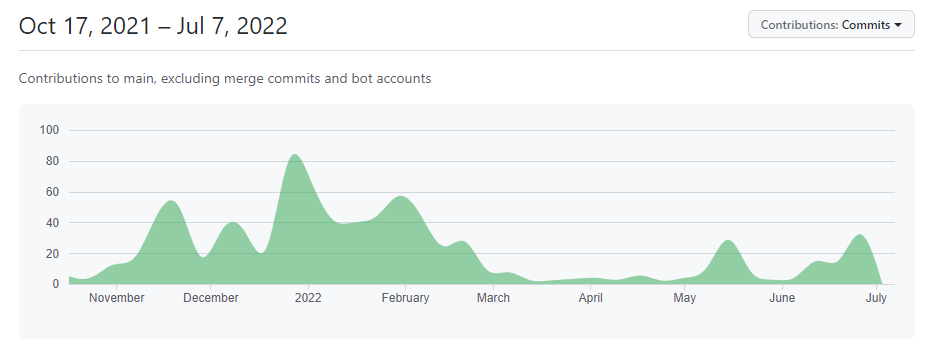
\includegraphics[width=\textwidth]{img/A/contribuciones.png}
    \caption{Contribuciones del Proyecto}
    \label{fig:A:contribuciones_del_proyecto}
\end{figure}

El proyecto se ha dividido en 5 Épicas:
\begin{itemize}
    \item \textbf{Spotify Frontend:} Esta épica contiene todas las tareas relacionada con el gestor de biblioteca / playlists / álbumes de Spotify. 
    \item \textbf{Database Frontend:} Esta épica contiene todas las tareas relacionadas con la interacción con la base de datos desde el Frontend. Además, se ha utilizado esta épica para la comunicacióon general con el backend. 
    \item \textbf{Backend Principal:} Esta épica contiene todas las tareas relacionada con el Backend NextJS, como la autenticación, transacciones de la base de datos, SSR, o comunicación con el analizador de tareas.
    
    \item \textbf{Analizador de Canciones:} Esta épica contiene todas las tareas relacionadas con el analizador de canciones, desde la investigación de técnicas y modelos, entrenamiento y experimentación con modelos hasta la implementación del backend. 
\end{itemize}

\subsection{Sprints}
Este apartado contine las distintas tareas organizadas por Sprints. No ha sido posible añadir una gráfica con el burndown debido a que Zenhub no permite generar el gráfico para los sprints anteriores a febrero. 

\subsubsection{Sprint 1}
\textbf{13/10/21 - 26/10/21}

\begin{itemize}
    \item Requisitos Funcionales. Coste inicial 1 punto, coste final  8 puntos. 
    \item Requisitos No Funcionales. Coste inicial  2 puntos, coste final 2 puntos.
    \item Buscar proveedores de Cloud. Coste inicial 2, Coste final 2.
    \item Diagrama de casos de uso. Coste inicial 3 puntos, coste final 8 puntos.
    \item Crear guía de estilo. Coste inicial 1 punto, coste final de 1 punto.
\end{itemize}


\subsubsection{Sprint 2}
\textbf{30/10/21 - 12/11/21}

\begin{itemize}
    \item Botón cambiar el Tema. Coste inicial 2, coste final 2.
    \item Diseño de la caché local. Coste inicial 2, coste final 2.
    \item Contexto de la API de Spotify, para que el cliente sea accesible desde todos los punto. Coste inicial de 2 puntos, coste final de 2 puntos. 
    \item Rutas Protegidas. Wrapper que impide a un usuario sin ciertas características acceder a ciertas rutas (por ejemplo /admin). Coste inicial 1 punto, coste final de 1 punto.
\end{itemize}


\subsubsection{Sprint 3}
\textbf{13/11/21 - 26/11/21}

\begin{itemize}
    \item Inicio de Sesión y Gestor de Cookies. Implementación del inicio de sesión y persistencia de credenciales en cookies. Coste inicial 8 puntos, coste final 8 puntos. 
    \item Caché Local. Se ha creado una caché local con DexieDB. Coste inicial 3, coste final 3. 
    \item Modal. Se ha creado un componente modal que contiene una vista anidad. Coste inicial 3, coste final 3.
    \item Track Card + Proxy de Carga. Se ha creado el componente carta que muestra una canción. Coste inicial 4, coste final 4. 
    \item Vista Genérica de Cartas. Se ha creado una vista genérica de cartas que pueda representar de forma eficiente cualquier tipo de tarjeta (canciones, álbumes, playlists o artistas). Coste inicial 8+5, coste final 8+5.
    \item Clientes REST Spotify y Lastfm. Coste inicial 2, coste final 2.
    \item Selector de Canciones para Playlist. Coste inicial 3, coste final 3.
    \item Implementación de los dátos homogéneos de Spotify. Coste inicial 2, Coste final 2. 
    
\end{itemize}



\subsubsection{Sprint 4}
\textbf{27/11/21 - 10/12/21}

\begin{itemize}
    \item Actualizar la versión de Typescript. Este cambio obligó a refactorizar los $catch$ ya que ahora necesitan estar tipados. Coste inicial 2, coste final 2.
    \item Configuración inicial de las acciones de Github para los tests de Jest. 
    \item Vista detallada de canciones. Coste inicial 3, coste final 3.
    \item Inicio de los filtros avanzados. 
    \item Inicio de la página de Inicio. Permite cargar las canciones y artistas favoritos del usuario. 
    \item Vista de artistas. Coste inicial 3, coste final 3. 
    \item Tarjeta de Artistas. Coste inicial 3, coste final 3. 
\end{itemize}


\subsubsection{Sprint 5}
\textbf{11/12/21 - 24/12/21}

\begin{itemize}
    \item Cambio en las proporciones de los botones para un diseño responsive. Coste inicial 1, coste final 1.
    \item Finalizado la integración de JEST con Github Actions. Coste inicial 2, coste final 2.
    \item Finalizados los filtros avanzados. Coste inicial 5, coste final 9.
\end{itemize}


\subsubsection{Sprint 6}
\textbf{11/12/21 - 24/12/21}

\begin{itemize}
    \item Terminar Home Page, integrando las distintas vistas. Coste inicial 2, coste final 13.
    \item Caché Manager. Implementación de la fachada como Hook de react. Coste inicial 5, coste final 5.
    \item Mejorar el rendimiento de la fachada. Las peticiones se realizan en paralelo. Coste inicial 
    \item Sistema de Notificaciones Genérico. Coste inicial 5, coste final 5.
    \item Caché de Notificaciones. Coste inicial 5, coste final 5. 
    \item Vista de Playlist. Coste inicial 5, coste final 5.
    \item Implementación de JWT. Coste final 5, costes final 5.
    \item Implementación de Vista de Estadísticas. Coste inicial 8, coste final 8.
    \item Detalles de Playlist. Coste inicial 5, coste final 5.
\end{itemize}


\subsubsection{Sprint 7}
\textbf{8/01/22 - 21/01/22}

\begin{itemize}
    \item Estado de la Fachada mediante un spinner. Coste inicial 2, coste final 2.
    \item Menú de navegación de Escritorio. Coste inicial 5. Coste final 8.
    \item Barra de navegación móviles. Coste inicial 5, coste final 5.
    \item Página de Opciones. Coste inicial 8. Coste final 8.
    \item Reproductor / Suena Ahora. Coste inicial 8, coste final 8.
    \item Selector de lenguaje. Coste inicial 4, coste final 4.
\end{itemize}

\subsubsection{Sprint 8}
\textbf{22/01/22 - 04/02/22}
\begin{itemize}
    \item Cliente de la base de datos. Coste inicial 4, coste final 4.
    \item Implementación de transacciones de etiquetas. Coste inicial 3, coste final 3.
    \item Exposición de las etiquetas mediante API REST. Coste inicial 3, coste final 3.
    \item Documentar la especificación de la API mediante OpenAPI. Coste inicial 1, coste final 1.
    \item Test de las APIs mediante Cypress. Coste inicial 3, coste final 3. 
    \item Solucionar el cambio de la URL de la API al cambiar el idioma. Coste inicial 1, coste final 1.
    \item Solucionar problemas de re-renderizado indeseados. Coste inicial 3, coste final 3.
    
    \item Vista de álbumes. Coste inicial 3, coste final 3.
\end{itemize}







\subsubsection{Sprint 9}
\textbf{05/02/22 - 18/02/22}
\begin{itemize}
    \item Detalles de álbumes. Coste inicial 2, coste final 2. 
    \item Gestor de Álbumes. Coste inicial 8, coste final 8.
    \item Editor de etiquetas de álbumes. Coste inicial 3, coste final 3.
    \item Investigar sobre técnicas de clasificación musical. Coste inicial 4, coste final 4.
    \item Demo de clasificador con Keras y Gtzan. Coste inicial 8, coste final 8.
    \item Página de Búsqueda. Coste inicial 5, coste final 5.
    \item Investigar técnicas y resultados de audio augmentation. Coste inicial 2, coste final 2.
    \item Ocular el fondo del modal con CSS. Coste inicial 1, coste final 1.
\end{itemize}


\subsubsection{Sprint 10}
\textbf{19/02/22 - 04/03/22}
\begin{itemize}
    \item Entrenar GTZAN a partir de modelos preentrenados. Coste inicial 5, coste final 5.
    \item Añadir vistas anidadas en los detalles. Coste inicial 8, coste final 8.
    \item Desarrollo de una aplicación en Node que permita descargar canciones de la API de Spotify. Coste inicial 3, coste final 5.
    \item Extensión del conjunto de datos GTZAN con 200 canciones más por cada género. Coste inicial 5, coste final 8. 

\end{itemize}

\subsubsection{Sprint 11}
\textbf{12/03/22 - 01/04/22}

\begin{itemize}
    \item Normalización de Playlist mediante Node. Coste inicial 3, coste final 3.
    \item Modelado del Dataset que incluya subgéneros. Coste inicial 1, coste final 1.
    \item Obtención de las etiquetas de Discogs. Coste inicial 2, coste final 2.
    \item Investigar Gtzan con técnias de clustering mediante DB SCAN y Kmeans. Coste inicial 2, coste final 2.
    \item Herramienta que extraiga los MFCCs y los almacene en fichero .npy. Coste inicial 2, coste final 2.
    \item Creación del Ludwig Dataset. Coste inicial 13, coste final 13.
\end{itemize}


\subsubsection{Sprint 12}
\textbf{2/04/22 - 22/04/22}
\begin{itemize}
    \item Implementación de una OVA para mejorar el resultado del clasificador en Ludwig. Coste inicial 13, coste final 13.
    \item Eliminar Reggae como género principal. Coste inicial 1, coste final 1.
    \item Implementar una arquitectura OVO de 32 CNNs para mejorar el rendimiento del clasificador. Coste inicial 3, coste final 8.
    \item Implementar Adaboost para mejorar el rendimiento. Coste inicial 3, coste final 3.
    \item Clasificar la salida de CNN mediante SVM para mejorar el rendimiento. Coste inicial 3, coste final 3.
    \item Entrenar todos los subgéneros. Coste inicial 5, coste final 5.
    \item Entrenar una OVA como clasificador de estados de ánimo. Coste inicial 8, coste final 8.
    
    \item Iniciar el Backend de MIR. Coste inicial 2.
    
\end{itemize}

\subsubsection{Sprint 13}
\textbf{23/04/22 - 06/05/22}
\begin{itemize}
    \item Implementar el motor de inferencia basado en ONNX. Coste inicial 5, coste final 5.
    \item Terminar el Backend de MIR. Coste final 8.
    \item Mejorar el rendimiento mediante inferencia en bloque. Coste inicial 3, coste final 3. 
    \item Configurar la integración continua de GCP Run par que publique el Backend MIR. Coste inicial 2, coste final 2.
    \item Sistema de recomendación basado en contenidos. Coste inicial 8, coste final 8.
    \item Sistema de recomendación colaborativo. Coste inicial 8, coste final 8.
\end{itemize}

\subsubsection{Sprint 14}
\textbf{07/05/22 - 20/05/22}
\begin{itemize}
    \item Integración Backend MIR con Frontend. Coste inicial 12, coste final 16.
    \item Cuantización de Modelos para reducir el consumo de memoria. Coste inicial 1, coste final 1.
    \item Internacionalización completa al castellano. Coste inicial 8, coste final 8. 
\end{itemize}


\subsubsection{Sprint 15}
\subsubsection{Sprint 14}
\textbf{21/05/22 - 03/06/22}
\begin{itemize}
    \item Desarrollo de los conceptos teóricos. Coste inicial 8, coste final 8.
    \item Protección del backend MIR mediante un código secreto. Coste inicial 3, coste final 3.
    \item Actualización de Estadísticas para incluir estados de ánimo. Coste inicial 3, coste final 3.
\end{itemize}


\subsubsection{Sprint Final}
\textbf{03/06/22 - 07 / 07 / 22}
\begin{itemize}
    \item Documentación de técnicas y herramientas. Coste inicial 8, coste final 8.
    \item Documentación de aspectos relevantes. Coste inicial 8, coste final 8.
    \item Documentación de Objetivos. Coste inicial 1, coste final 1.
    \item Documentación de Introudcción y Abstract. Coste inicial 1, coste final 1.
    \item Creación de Docker Compose. Coste inicial 4, coste final 4.
    \item Crear página de inicio. Coste inicial 4, coste final 4.
    \item Finalizar anexos de diseño y requisitos. Coste inicial 8, coste final 8.
    \item Crear una vista de sistema mediante Figma. Coste inicial 2, coste final 2.
    \item Documentación del Plan de Proyecto. Coste inicial 8, coste final 8.
\end{itemize}



\section{Estudio de viabilidad}

En este apartado se va realizar un estudio sobre la viabilidad económica y legal del proyecto, teniendo en cuenta distintos apartados como los

\subsection{Viabilidad económica}

El proyecto no es económicamente viable ya que los términos y condiciones de Spotify \cite{Spotify_terms:online} y LastFM \cite{A:Last_APITerms18:online}. Estos servicos solo permiten utilizar la API pública para \textbf{uso personal}, por lo que no se puede monetizar.

\subsubsection{Costes}

En esta sección se van a desglosar y analizar los distintos costes del proyecto.

\textbf{Costes de Hardware}

Los únicos costes hardware son un ordenador portátil junto con sus periféricos.

Suponiendo que la vida útil de un ordenador portátil son 6 años podemos estimar su coste amortizado durante el primer año. Estos costes están desglosados en \ref{A:tab:hardware}

\begin{table}[H]
\centering{%

    \begin{tabular}{@{}lll@{}}
    \toprule
    Concepto               & Coste (€) & Amortización (€) \\ \midrule
    Portátil y Periféricos & 850       & 631              \\ \midrule
    Total                  & 850     & 631                 \\ \bottomrule
    \end{tabular}%
    }
    \caption{Costes Hardware}
    \label{A:tab:hardware}
\end{table}

\textbf{Costes Fijos de Software}

En este apartado \ref{A:tab:fijos} se van a analizar los costes anuales de los distintos servicios y suscripciones. 

\begin{table}[H]
\centering{%
    \begin{tabular}{@{}lll@{}}
    \toprule
    Concepto               & Coste (€) & Amortización (€) \\ \midrule
    Vercel\footnote{Alojamiento de la Web} & 240       & 163.7            \\
    Codacy & 170       & 113           \\ 
    Github Premium &   48     & 32.2           \\ 
    Github Copilot & 120      & 163.7            \\ \midrule
    Total                  & 578    & 488.4               \\ \bottomrule
    \end{tabular}%
    }
    \label{A:tab:fijos}
    \caption{Costes Fijos}
\end{table}

\textbf{Costes por Usuario}

Según los análisis de Google Cloud Platform, el coste medio por usuario por usuario para cada uno de los servidores webs son unos 13.26 céntimos al mes, siendo el servidor web de análisis de canciones el más cara de mantener por los altos tiempos de ejecución y consumos de memoria. 

AWS DynamoDB tiene un coste mensual de 0.072 céntimos por cada unidad de lectura y escritura en la base de datos, y un coste de 0.283 céntimos por cada GB/mes. Se estima que es necesaria 1 unidad de lectura y escritura por cada 10000 usuarios. Cada canción almacenada tiene un tamaño medio de 412 Bytes y cada usuario almacena de media 1.2KB en etiquetas. \\
Serían necesarios 200 millones de usuarios (más usuarios que suscriptores de Spotify \cite{A:spot_subs}) o 625 millones de canciones almacenadas. Como es prácticamente imposible alcanzar estos números de usuarios o canciones, se ha decidido obviar el coste del almacenamiento debido a que el uso comercial entra dentro del plan gratuito de AWS. 

Podemos estimar que el coste por usuario es de unos \textbf{14 céntimos al mes}. Además, a medida que se analicen más canciones, es posible que el coste se vea reducido debido al aumento de lecturas en la base de datos y el menor uso del analizador de canciones. 

\textbf{Costes Personal}

Para este coste se va a tener en cuenta el coste de un único empleado encargado del desarrollo, mantenimiento y soporte de usuario de la página web hasta que se decida dejar de dar soporte al servicio. 

En este caso se ha escogido un suelo base bruto de 21.000 euros, considerando el salario de un desarrollador junior fullstack sin apenas experiencia, que ha sido desglosado en \ref{A:salario}

\begin{table}[H]
    \centering{%
    \begin{tabular}{ll}
    \hline
    Concepto                                                                                                         & Coste (€) \\ \hline
    Salario Mensual Neto (12 pagas) &  1.425,4   \\
    Retenciones IRPF & 2.562,2 \\
    Cuotas Seguridad Social &  1.333,5 \\
    \hline
    Total & 21.000,0
    \\ \hline
    \end{tabular}%
    }
    \label{A:salario}
    \caption{Desglose Coste anual del Webmaster}
\end{table}

\textbf{Otros Costes}

La tabla \ref{A:otros_costes} contiene otros costes que han aparecido a lo largo del proyecto. 
\begin{table}[H]
    \centering{%
    \begin{tabular}{ll}
    \hline
    Concepto                                                                                                         & Coste (€) \\ \hline
    3 USBs &  14,5  \\
    Memoria & 23,5       \\
    \hline
    Total & 38,0\\
    \hline
    \end{tabular}%
    }
    \label{A:otros_costes}
    \caption{Coste anual del Webmaster}
\end{table}
\textbf{Coste Primer Año}

La tabla  \ref{A:coste_ano_1} contiene el coste del proyecto durante el primer año. 

\begin{table}[H]
    \centering{%
    \begin{tabular}{ll}
    \hline
    Concepto                                                                                                         & Coste (€) \\ \hline
    Salarios &  21.000,0   \\
    Licencias & 488,4 \\
    Hardware & 631 \\
    20 Usuarios & 3,33 \\                                                                 \hline
    Total & 22122.73 \\ 
    \hline
    \end{tabular}%
    }
    \label{A:coste_ano_1}
    \caption{Coste durante el primer año}
\end{table}

\subsection{Viabilidad legal}

En esta sección se va a analizar las distintas licencias de las dependencias, así como términos y condiciones de las APIs que hemos utilizado. 

\subsubsection{Api de Spotify}
La api de Spotify detalla sus términos y condiciones en \cite{A:SpotifyTerms:online}. Los términos más importantes están reflejados en la tabla \ref{tab:A:spotify_terms}.

\begin{table}[h]
    \resizebox{\textwidth}{!}{%
    \begin{tabular}{@{}ll@{}}
        \toprule
        Condición                                                                                                                                                  & Estado \\ \midrule
        Uso No Comercial                                                                                                                                           &   \checkmark   \\
        \begin{tabular}[c]{@{}l@{}}No se almacenan datos de Spotify \\ que puedan quedarse obsoletos\end{tabular}                                                  & \checkmark        \\
        \begin{tabular}[c]{@{}l@{}}Los resultados tienen en cuenta el mercado\\ del usuario / no permite a usuarios saltarse restricción geográficas.\end{tabular} & \checkmark        \\
        \begin{tabular}[c]{@{}l@{}}La plataforma cumple con las recomendaciones\\  de la guía de diseño de Spotify\end{tabular}                                    &\checkmark         \\
        No se modifican los metadatos de Spotify                                                                                                                   & \checkmark        \\
        No se utiliza la API para uso malicioso                                                                                                                    & \checkmark        \\
        No se daña la imagen de Spotify                                                                                                                            & \checkmark        \\
        Incumplimiento de la propiedad intelectual                                                                                                                 & \checkmark        \\
        \begin{tabular}[c]{@{}l@{}}Se oculta la implementación de características $Premium$ a\\
        usuarios que no son suscriptores\end{tabular}                      &  \checkmark       \\ 
        No se cachean los resultados de la API & \textbf{\~}\\

        \bottomrule
    \end{tabular}%
    }
    \label{tab:A:spotify_terms}
    \caption{Términos y Condiciones más importantes de la API de Spotify}
\end{table}


El punto más interesante es la sección IV apartado 3b, que prohíbe el uso de caches. Si detallamos este punto se puede observar como únicamente se permite el uso de cachés si \textbf{se utilizan para el rendimiento}, \textbf{son temporales}. SpotMyFM cumple con ambos casos de uso.

\subsubsection{Api de LastFM}

Los términos y condiciones de la API pública de LastFM pueden encontrarse en \cite{A:Last_APITerms18:online}.
En este caso, se pueden resaltar los términos y condiciones en la siguiente tabla \ref{A:last_terms}.

\begin{table}[H]
    \centering{%
    \begin{tabular}{ll}
    \hline
    Condición                                                                                                           & Estado \\ \hline
    Se acredita el origen de los datos a LastFM                                                                         &  \checkmark      \\
    Uso No Comercial                                                                                                    &  \checkmark       \\
    No se licencian los datos de LastFM                                                                                 &    \checkmark    \\
    \begin{tabular}[c]{@{}l@{}}No se modifican los datos de LastFM de\\ manera que dañe la imagen de marca\footnote{No se han modificado los datos de ninguna manera.}\end{tabular} &  \checkmark      \\ \hline
    \end{tabular}%
    }
    \label{A:last_terms}
    \caption{Términos y Condiciones más importantes de la API de LastFM}
\end{table}
En este caso se han cumplido con todos los requisitos que especifican los términos y condiciones de la API. 

\subsubsection{Licencias Software}
Una licencia software es una definición legal vinculante que indica los límites y condiciones para el uso de cada una de las dependencias. Cada dependencia puede tener un tipo de licencia distinto, por lo que es necesario revisar si algunas de las licencias es incompatible con el proyecto. 

Las licencias de cada una de las dependencias han sido detalladas en \ref{tab:A:Licencias}. Todas las licencias admiten los distintos usos que va a tener el producto.  

\begin{table}[H]
    \centering
    \begin{tabular}{ll}
    \hline
        Dependencia & Licencia \\
         Babel & MIT \\
         Cypress & MIT y Apache \\
         Jest & MIT \\
         npmcli & ISC \\
         popperjs & MIT \\
         @uiball/loader & MIT \\
         axios & MIT \\
         base64 & MIT \\
         dexie & Apache 2.0 \\
         dotenv & BSD-2-Clause \\
         Framer Motion & MIT \\
         js-cookies & MIT \\
         jsonwebtoken & MIT \\
         lodash & MIT \\
         next & MIT \\
         next-translate & MIT \\
         pretty-ms & MIT\\
         react-device-detect & MIT \\
         react-dom & MIT \\
         react-icons & MIT \\
         react-switch & MIT \\
         react-is & MIT \\
         react-toastify & MIT \\
         react-use & MIT \\
         recharts & MIT \\
         spotify-web-api-js & MIT \\
         spotify-web-api-node & MIT \\
         styled-components & MIT \\
         tiny-async-pool & MIT \\
         twin.macro & MIT \\
         estlint & MIT \\
         ONNX & Apache 2.0 \\
         FastAPI & MIT \\
         Tensorflow & Apache 2.0 \\
         Python & PSFN\footnote{Python Software Foundation License, compatible con GPL} \\
         
         
    \hline
    \end{tabular}
    \caption{Licencias}
    \label{tab:A:Licencias}
\end{table}

\apendice{Especificación de Requisitos}

\section{Introducción}

\section{Objetivos generales}

\section{Catalogo de requisitos}

\subsection{Requisitos funcionales}\label{requisitos-funcionales}
\begin{itemize}
\tightlist

    \item
        \textbf{RF-1 Gestión de Biblioteca:} Se requiere que la web sea capaz de mostrar la biblioteca de música personal del usuario.
        \begin{itemize}
           \tightlist
           
            \item
                \textbf{RF-1.1 Listar Biblioteca:} Se requiere que el usuario pueda visualizar su biblioteca de usuario
                \begin{itemize}
                    \item
                        \textbf{RF-1.1.1 Filtrar Vista:} Se requiere que el usuario pueda filtrar la vista de su biblioteca mediante filtros avanzados.
                    \item
                        \textbf{RF-1.1.2 Seleccionar Vista:} Se requiere que el usuario pueda marcar como seleccionados los elementos filtrados.
                    \item
                        \textbf{RF-1.1.3 Ordenar Vista:} Se requiere que el usuario pueda ordenar la vista actual a partir de parámetros.
                    \item
                        \textbf{RF-1.1.3 Detallar Canción:} Se requiere que el usuario pueda ver detalles de cualquier item de la vista. 
                \end{itemize}
                
            \item
                \textbf{RF-1.2 Crear de Playlists:} Se requiere que el usuario pueda crear playlists a partir de una selección de canciones.   
                \begin{itemize}
                    \item 
                        \textbf{RF-1.2.1 Configurar Playlist:} Se requiere que el usuario pueda escoger el título, descripción y opciones de privacidad de cada playlist.
                    \item 
                        \textbf{RF-1.2.2 Dividir Playlist:} Se requiere que el usuario pueda dividir una playlist en múltiples playlists.
                \end{itemize}
                
            \item
                \textbf{RF-1.3 Ampliar Playlists:} Se requiere que el usuario pueda ampliar sus playlists ya creadas a partir de una selección de canciones.
                \begin{itemize}
                    \item
                        \textbf{RF-1.3.1 Buscar Playlist:} Se requiere que el usuario pueda seleccionar su playlist a partir de un listado.
                    \item
                        \textbf{RF-1.3.2 Detallar Playlist:} Se requiere que el usuario pueda ver los detalles de una playlist.
                \end{itemize}
        \end{itemize}
    

        
    \item  
        \textbf{RF-2 Gestión de Álbumes:} Se requiere que la web sea capaz de mostrar los álbumes del usuario.
        \begin{itemize}
            \item 
                \textbf{RF-2.1 Listar Álbumes:} Se requiere que el usuario pueda visualizar sus álbumes.
                \begin{itemize}
                    \item 
                        \textbf{RF-2.1.1 Álbumes Favoritos:} Se requiere que el usuario pueda visualizar sus álbumes marcados como favoritos.
                    \item 
                        \textbf{RF-2.1.2 Álbumes Etiquetados:} Se requiere que el usuario pueda visualizar sus álbumes etiquetados.
                        
                    \item
                        \textbf{RF-2.1.3 Filtrar Vista:} Se requiere que el usuario pueda filtrar la vista actual de sus álbumes mediante filtros avanzados.
                    \item
                        \textbf{RF-1.1.3 Ordenar Vista:} Se requiere que el usuario pueda ordenar la vista actual a partir de parámetros.
                    \item
                        \textbf{RF-1.1.3 Detallar Álbum:} Se requiere que el usuario pueda ver detalles de cualquier álbum en la vista. 
                \end{itemize}
                
            \item 
                \textbf{RF-2.2 Buscar Álbumes:} Se requiere que el usuario pueda visualizar álbumes a partir de una cadena.
            \item
                \textbf{RF-2.3 Gestionar Álbumes Favoritos:} Se requiere que el usuario pueda marcar o desmarcar cualquier álbum como favorito.
            \item
                \textbf{RF-2.4 Etiquetar Álbumes:} Se requiere que el usuario Añadir etiquetas a cualquier álbum.
                \begin{itemize}
                    \item 
                    \textbf{RF-2.4.1 Etiquetas Personalizadas:} Se requiere que el usuario pueda crear sus propias etiquetas.
                \end{itemize}
        \end{itemize}

    \item
        \textbf{RF-3 Detallar Elementos:} Se requiere que el usuario pueda ver detalles de un álbum, playlist o seleccionado por el usuario.
            \begin{itemize}
                \item 
                \textbf{RF-3.1 Detallar Canción:} Se requiere que el usuario pueda ver detalles de una canción específica.
                    \begin{itemize}
                        \item 
                            \textbf{RF-3.1.1 Previsualizar Canción:} Se requiere que el usuario pueda escuchar un fragmento de la canción.
                        \item
                            \textbf{RF-3.1.2 Analizar Canción:} Se requiere que el usuario pueda obtener detalles especiales a partir de un análisis de un fragmento de la canción.
                        \item
                            \textbf{RF-3.1.3 Reproducir Canción:} Se requiere que el usuario pueda reproducir o añadir a la cola una canción en un cliente de Spotify.
                        \item
                            \textbf{RF-3.1.4 Detallar Álbum:} Se requiere que el usuario obtenga los detalles del álbum al que pertenece dicha canción.

                    \end{itemize}
                    
                \item 
                \textbf{RF-3.2 Detallar Álbum:} Se requiere que el usuario pueda ver detalles de un álbum específico.
                    \begin{itemize}
                        \item 
                            \textbf{RF-3.2.1 Gestionar Etiquetas:} Se requiere que el usuario pueda visualizar o gestionar las etiquetas de un álbum
                        \item 
                            \textbf{RF-3.2.2 Conocer Estadísticas:} Se requiere que el usuario pueda ver las estadísticas del álbum mediante LastFM.
                        \item 
                            \textbf{RF-3.2.3 Reproducir Álbum:} Se requiere que el usuario pueda reproducir el álbum en un cliente Spotify.                 
                        \item 
                            \textbf{RF-3.2.3 Detallar Artistas:} Se requiere que el usuario pueda conocer los detalles de los artistas que han participado en el álbum.
                    \end{itemize}
                
                \item
                    \textbf{RF-3.3 Detallar Artistas:} Se requiere que el usuario pueda conocer los detalles de un artista en específico.
                    \begin{itemize}
                        \item \textbf{RF-3.3.1 Géneros Musicales} Se requiere que el usuario pueda conocer los géneros musicales de un artista. 
                    \end{itemize}
            \end{itemize}

    \item
        \textbf{RF-4 Gestión de Tema:} Se requiere que el usuario pueda cambiar el tema actual en cualquier punto de la web.
            \begin{itemize}
                \item 
                \textbf{RF-4.1 Tema Persistente:} Se requiere que el tema seleccionado se mantenga entre sesiones. 
            \end{itemize}
            
    \item
        \textbf{RF-5 Gestión de Sesión:} Se requiere que el usuario tenga el control de la sesión actual.
        \begin{itemize}
            \item
                \textbf{RF-5.1 Cerrar Sesión:} Se requiere que el usuario pueda cerrar su sesión desde la web.
                \begin{itemize}
                    \item
                    \textbf{RF-5.1.1 Limpieza de Sesión:} Se requiere que todos los datos locales sean borrados al cerrar sesión.
                \end{itemize}
            \item
                \textbf{RF-5.2 Limpiar Datos Locales:} Se requiere que los datos locales puedan borrarse desde la web.
        \end{itemize}
    
    \item
        \textbf{RF-5 Estadísticas:} Se requiere que el usuario pueda visualizar las estadísticas relacionadas con su cuenta.
        \begin{itemize}
            \item \textbf{RF-5.1 Listar Canciones}: Se requiere que el usuario pueda conocer sus canciones más escuchadas en diversos periodos de tiempo.
            \item \textbf{RF-5.2 Listar Artistas}: Se requiere que el usuario pueda conocer sus artistas más escuchadas en diversos periodos de tiempo.
        \end{itemize}
    
    \item
        \textbf{RF-6 Cachear Peticiones:} Se requiere que la aplicación realice el mínimo número de peticiones a la API para no sobrepasar los límites.
            \begin{itemize}
                \item \textbf{RF-6.1 Cachear Canciones:} Se requiere que los datos de las canciones se almacenen de forma local.
                \item \textbf{RF-6.2 Cachear Artistas:} Se requiere que los datos de los artistas se almacenen de forma local.
                \item \textbf{RF-6.3 Cachear Álbumes:} Se requiere que los datos de los álbumes se almacenen de forma local.
                \item \textbf{RF-6.4 Refrescar Caché:} Se requiere que los distintos datos almacenados puedan actualizarse para evitar inconsistencias.
            \end{itemize}
    \item
        \texbf{RF-7 Analizar Canciones:} Se requiere que el usuario pueda conocer detalles de cada una de las canciones a partir de un fragmento de la canción.
    
    
\end{itemize}

\subsection{Requisitos no funcionales}\label{requisitos-no-funcionales}
\begin{itemize}
    \item \textbf{RNF-1 Diseño Responsive:} Se requiere un diseño "responsive" para poder utilizarla en dispositivos con distintos tamaños de pantalla o relaciones de aspecto sin perder información.
    \item \textbf{RNF-2 Minimizar Peticiones:} Se requiere minimizar el número de peticiones posibles a las  distintas APIs para evitar alcanzar los límites ver \textbf{RF-6}). 
    \item \textbf{RNF-3 Internacionalización:} Se requiere que la web esté disponible en, al menos, dos idiomas. Algunos elementos como las fechas de lanzamiento deberán tener el formato de fecha adecuado. 
    
    \item\textbf{RNF-4 Compatibilidad:} Se requiere que la web sea funcional a lo largo de los motores webs más utilizados (Chromium, Firefox y Apple Webkit).
    \item\textbf{RNF-5 Carga Diferida:} Se requiere que la web evite cargar un exceso de datos si el usuario no va a necesitarlos, por ejemplo aplicando el patón de Carga Diferida para paginar la carga de imágenes.
    \item\textbf{RNF-6 Accesibilidad:} Se requiere que la web cumpla con el mayor número de recomendaciones posible de Web Content Accessibility Guidelines (WCAG) 2.1
    \item\textbf{RNF-7 Rendimiento y Buenas Prácticas: Se requiere que la web funcione correctamente en dispositivos móviles y en escritorio, minimizando el tamaño de la aplicación para acelerar las cargas de JavaScript y evitar las esperas en el navegador.}
    \item\textbf{RNF-8 Seo:} Se requiere que la web pueda ser indexada en distintos motores de búsqueda y si apliquen técnicas para mejorar la posición de esta.
    \item\textbf{RNF-9 Seguridad: Se requiere que la web sea segura, utilizando TSL o SSL y con actualizaciones constantes para evitar paquetes de terceros con vulnerabilidades.}
    \item\textbf{RNF-10 Privacidad: Se requiere almacenar el mínimo de información que puede identificar a un usuario para mejorar la privacidad de los datos.}
\end{itemize}





\section{Especificación de requisitos}

\subsection{Diagrama de Casos de Uso}

\subsection{Casos de Uso}


\begin{table}[]
\centering
\begin{tabular}{r|p{0.6\textwidth}}
\hline
\textbf{CU-01}         & \textbf{Gestionar Tema}                                 \\ \hline
\textbf{Versión}       & 1.0                                                     \\
\textbf{Autor}         & Jorge Ruiz Gómez                                        \\
\textbf{Requisitos}    & RF-4                                         \\
\textbf{Descripción}   & Permite al usuario cambiar el tema general de la página \\ \hline
\textbf{Precondición}  & Ninguna                                                 \\
\textbf{Acciones}      &    \begin{itemize}
                                \item El Usuario entra en la página.
                                \item La web carga el tema almacenado.
                                \item El usuario pulsa el botón de cambio de tema.
                                \item El Tema se alterna.
                                \item La selección del tema se almacena de forma local.
                            \end{itemize}\\
                                                                          
\textbf{Postcondición} & El tema ha cambiado                                     \\
\textbf{Excepciones}   & Ninguna                                                 \\
\textbf{Importancia}   & Baja                                                    \\ \hline
\end{tabular}
\caption{CU-01}
\label{tab:my-table}
\end{table}


\begin{table}[]
\centering
\begin{tabular}{r|p{0.6\textwidth}}
\hline
\textbf{CU-02}         & \textbf{Gestionar Tema}                                 \\ \hline
\textbf{Versión}       & 1.0                                                     \\
\textbf{Autor}         & Jorge Ruiz Gómez                                        \\
\textbf{Requisitos}    & RF-4                                         \\
\textbf{Descripción}   & Permite al usuario cambiar el tema general de la página \\ \hline
\textbf{Precondición}  & La página ha cargado                                                 \\
\textbf{Acciones}      &    \begin{itemize}
                                \item El Usuario entra en la página.
                                \item La web carga el tema almacenado o selecciona un por defecto.
                                \item El usuario pulsa el botón de cambio de tema.
                                \item El Tema se alterna.
                                \item La selección del tema se almacena de forma local.
                            \end{itemize}\\
                                                                          
\textbf{Postcondición} & El tema ha cambiado                                     \\
\textbf{Excepciones}   & Ninguna                                                 \\
\textbf{Importancia}   & Baja                                                    \\ \hline
\end{tabular}
\caption{CU-02}
\label{tab:my-table}
\end{table}










\apendice{Especificación de diseño}

\section{Introducción}

En este apartado se van a documentar las decisiones de diseño más relevantes del proyecto, como el diseño de datos o el diseño de clases de algunos componentes del sistema. 

\section{Diseño de Datos}
Para el diseño de datos se ha decidido utilizar el modelo relacional debido a su similitud con los esquemas clave-valor que se utilizan en la base de datos basadas en documentos.


\subsection{DynamoDB}

Se ha utilizado la base de datos NOSQL basada en documentos DynamoDB.\\
La base de datos contiene 5 tablas, de las cuales 2 son versiones destinadas a ejecutar los tests / desarrollo. Cada uno de los elementos de la base de datos contiene dos atributos obligatorios, $updated\_at$ y $created\_at$, estos atributos son strings que almacenan una fecha en formato ISO 8601. 

\subsubsection{LudwigDataset}
Esta tabla contiene todos los items del conjunto de datos Ludwig \ref{fig:C:dynamo_dataset}. La clave primaria (o clave de partición en DynamoDB), se identifica como $PK$, y es un string que almacena el id de la canción en Spotify. Por otro lado, se almacena el $MBID$ de Brainz, un valor único en toda la tabla. Discogs \cite{C:a2022_discogs} tiene muchos más subgéneros que los listados en la memoria, por ello se almacenan el resto de subgéneros que no se van a utilizar para entrenar los clasificadores en el campo $otherSubgenres$. Los estados de ánimo almacenan un valor entre 0 y 1 que indican la confianza de ese estado de ánimo. 

La obtención de este dataset se realiza siguiendo el proceso indicado en el diagrama de la figura \ref{fig:ludwig_dataset}

\begin{figure}
    \centering
    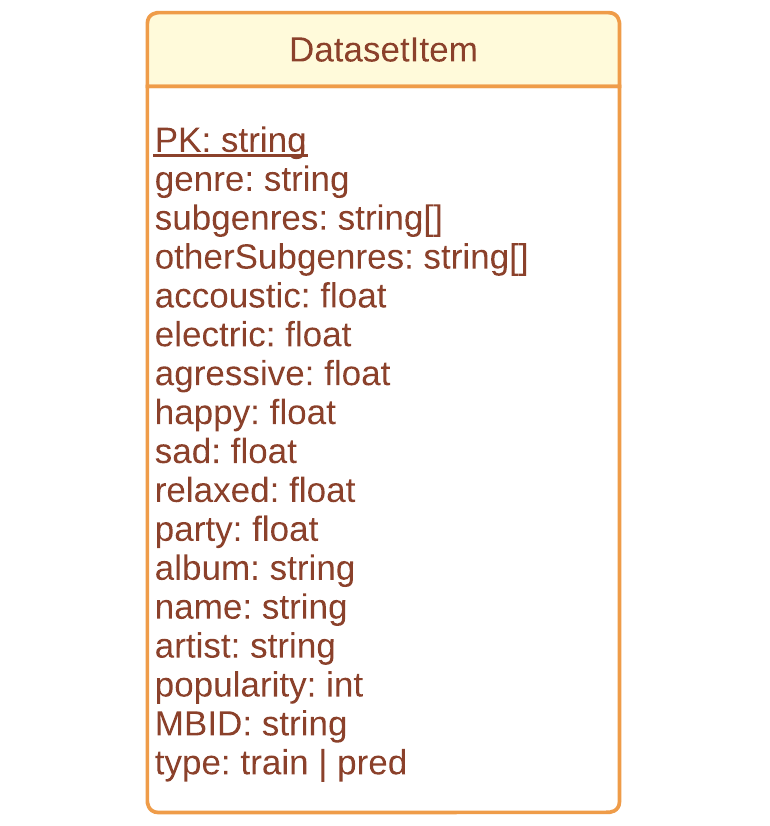
\includegraphics{img/C/data_dataset.png}
    \caption{DynamoDB: Ludwig Dataset}
    \label{fig:C:dynamo_dataset}
\end{figure}


\begin{figure}
    \centering
    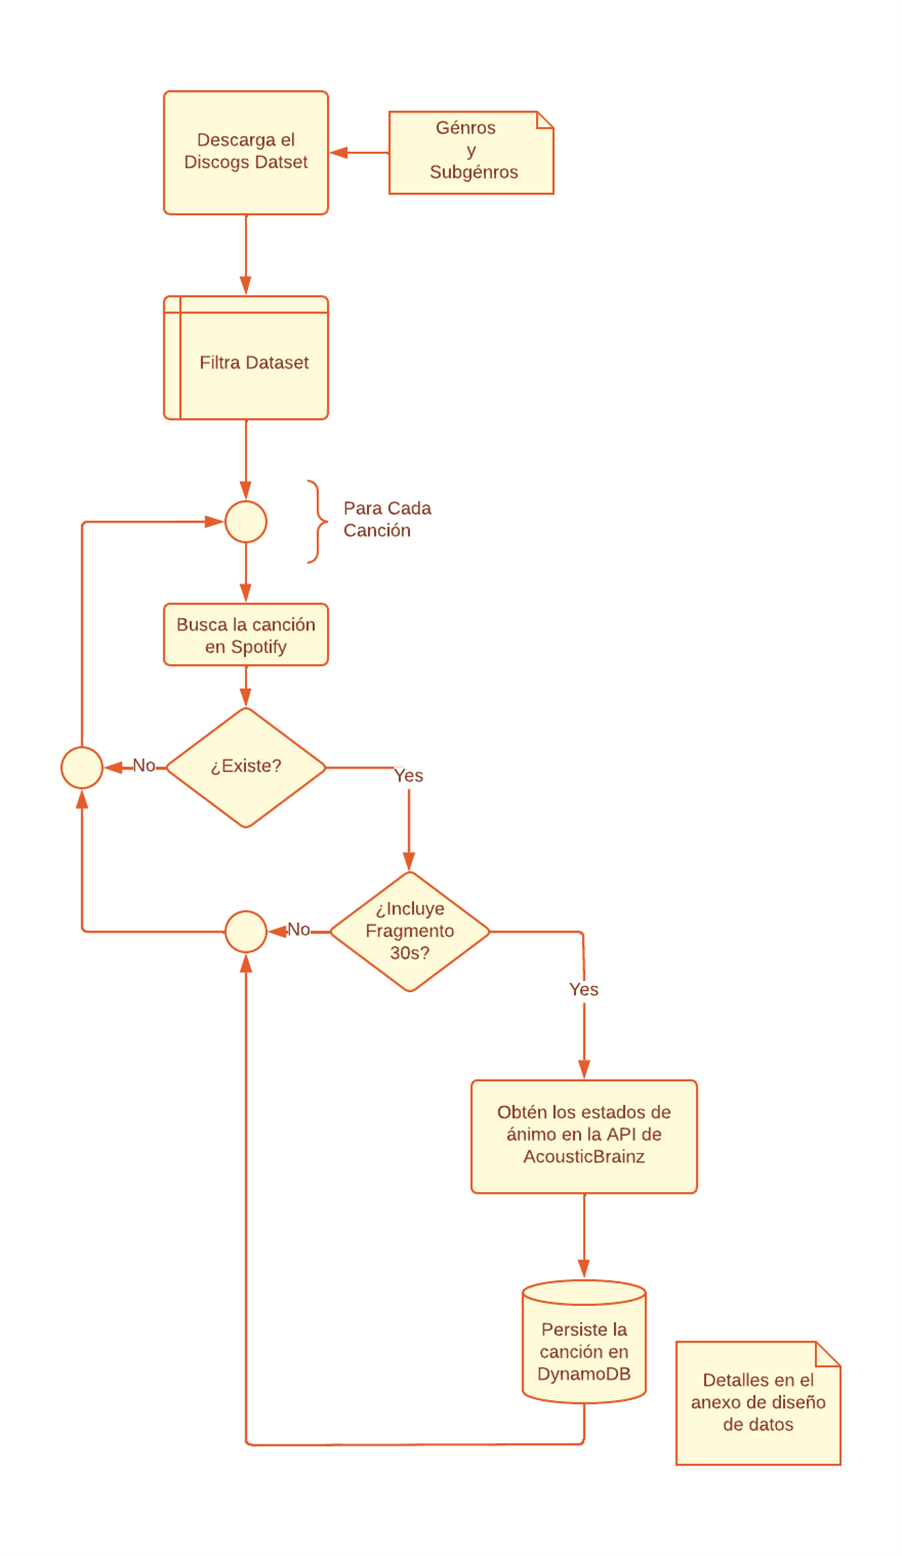
\includegraphics[width=12cm]{img/5/ludwig_dataset.png}
    \caption{Proceso de obtención de los datos de Ludwig Dataset}
    \label{fig:ludwig_dataset}
\end{figure}

\subsubsection{Tracks y Tracks\_test}
La tabla Tracks \ref{fig:C:dynamo_results} contiene los resultados del clasificador de géneros. \\
El identificador de la tabla, $PK$, almacena el id de Spotify de una canción. Esta tabla contiene un atributo $version$, que permite identificar la versión del clasificador, ya que si reemplazamos el modelo principal, es posible los resultados almacenados y los resultados del clasificador sean distintos.
La implementación de SpotMyFM obliga a DynamoDB a indexar $version$ para que únicamente se puedan obtener los resultados de la versión actual del clasificador.

\begin{figure}
    \centering
    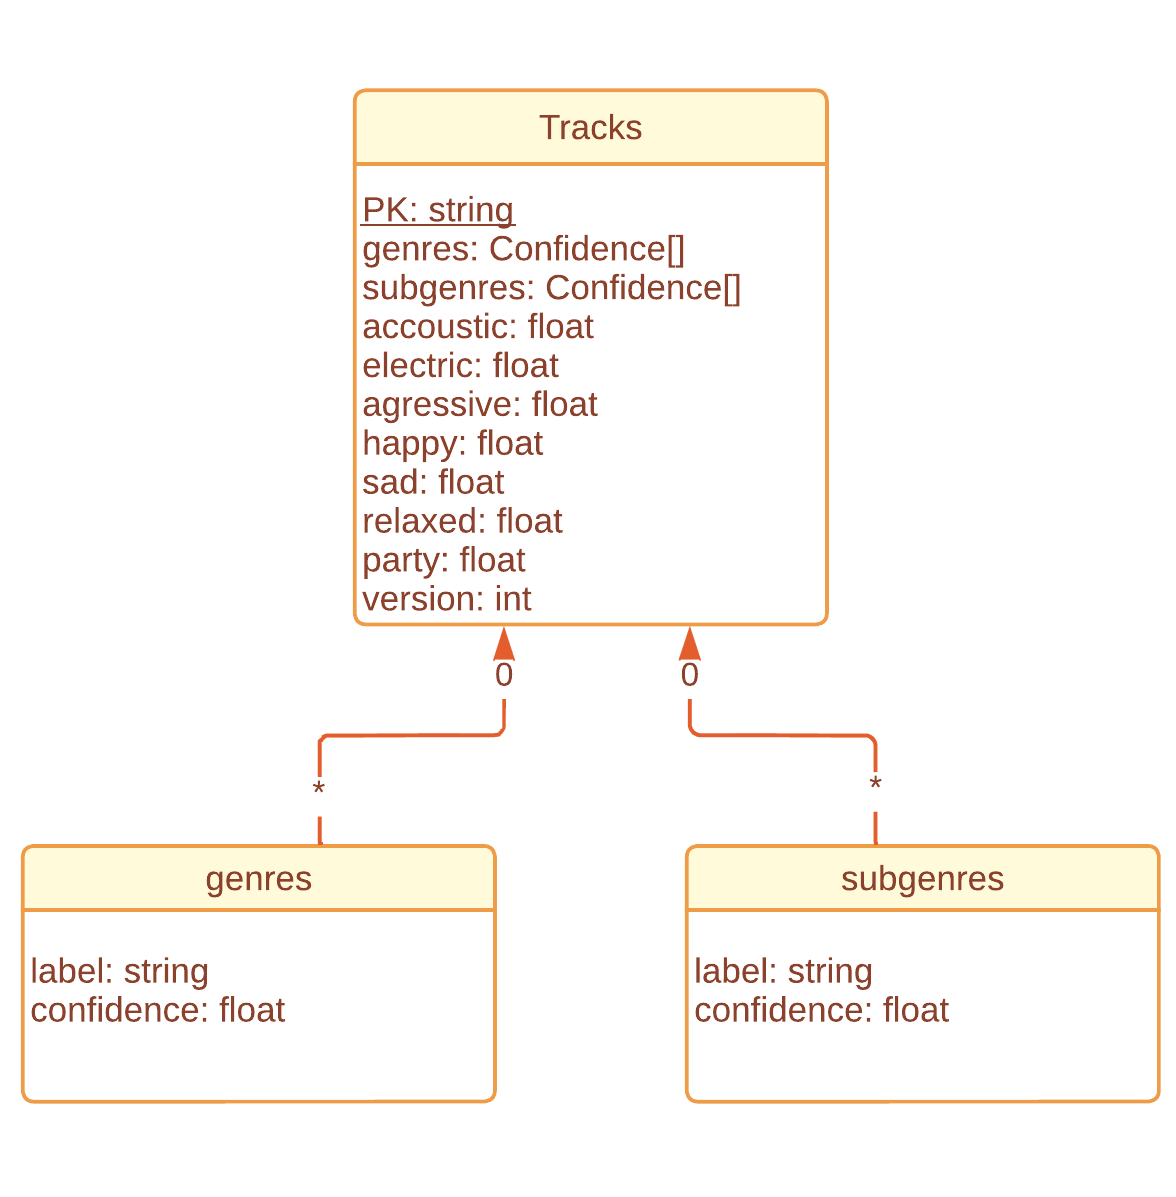
\includegraphics{img/C/data_tracks.png}
    \caption{DynamoDB: Resultados del analizador de canciones}
    \label{fig:C:dynamo_results}
\end{figure}

\subsubsection{Users y Users\_test}
La tabla Users \ref{fig:C:dynamo_users} contiene la información de los usuarios que han utilizado la función de etiquetas de SpotMyFM. Debido a la limitación de DynamoDB de 40kB por cada atributo, debemos almacenar las etiquetas asociadas a cada álbum mediante atributos dinámicos. Estos campos no se pueden declarar en Dynamoose, por lo que si queremos identificar que un campo es de un tipo específico, es necesario asignarle un prefijo, como por el ejemplo $ALB:<id\_album>$, donde $<id\_album>$ hace referencia al ID de Spotify del álbum.
\begin{figure}[]
    \centering
    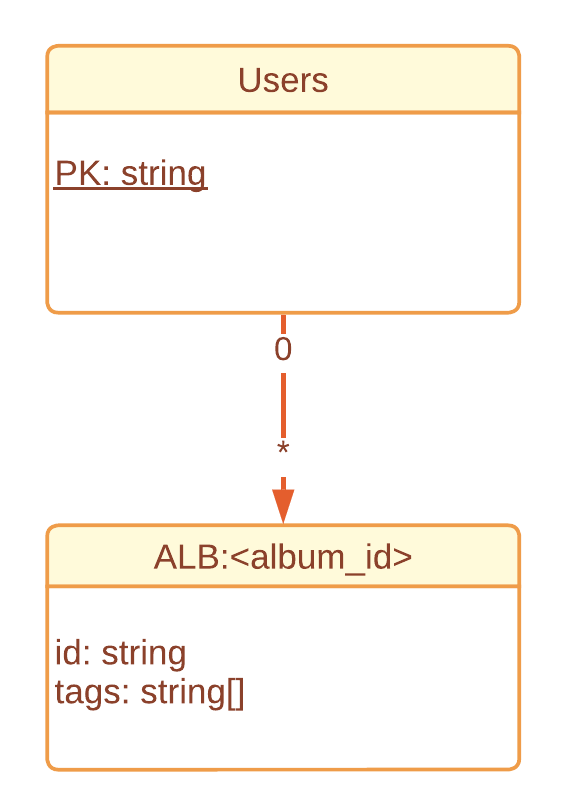
\includegraphics{img/C/data_users.png}
    \caption{DynamoDB: Tabla usuarios}
    \label{fig:C:dynamo_users}
\end{figure}

\clearpage

\subsection{Datos del Frontend} \label{C:datos_front}

Una de las fuentes de datos de la capa \textbf{modelo} \ref{modelo_vista_presentador} es DexieDB \ref{fig:c:dexie}, una base de datos NOSQL que utilizamos como caché intermedia para almacenar los datos obtenidos de las distintas fuentes de datos. 

Se ha diseñado el siguiente esquema relacional \ref{fig:c:dexie} mediante interfaces de Typescript. En este caso una canción está compuesta por un único álbum y uno o más artistas. Cada álbum está compuesto por uno o más artistas.

\begin{figure}
    \centering
    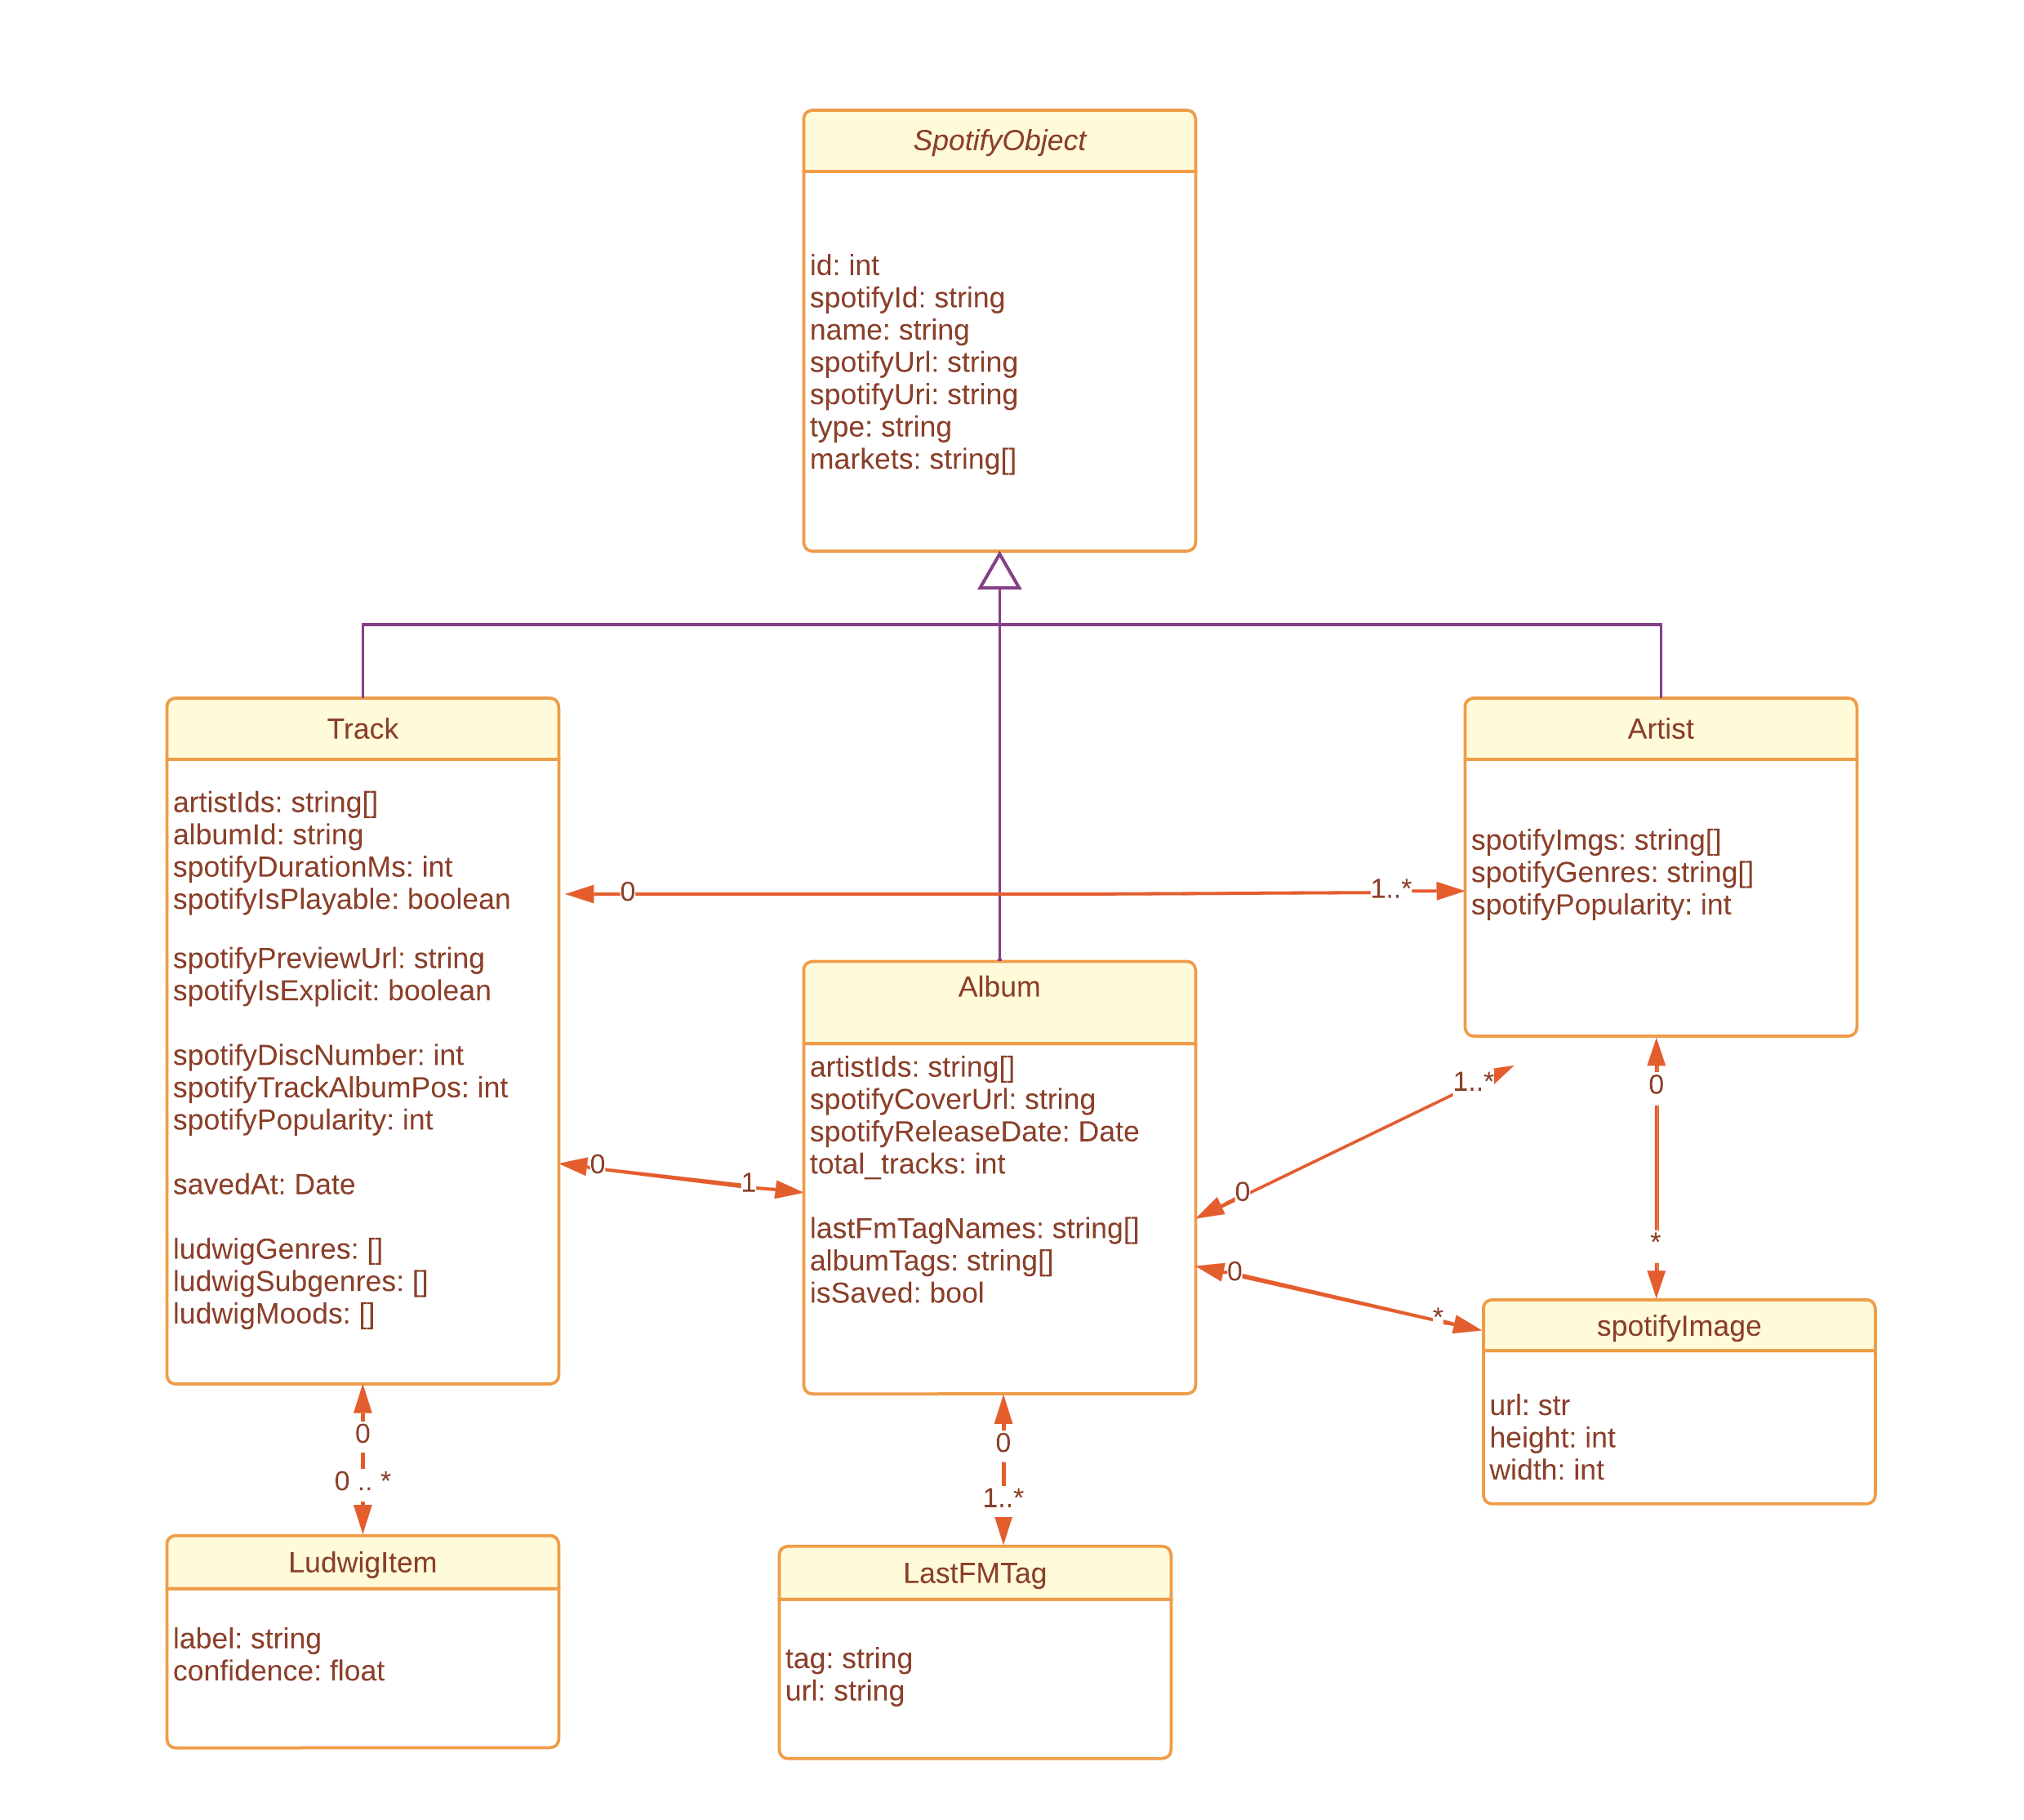
\includegraphics[width=\linewidth]{img/C/data_cache.png}
    \caption{DexieDB: Canciones, álbumes y artistas}
    \label{fig:c:dexie}
\end{figure}



\section{Diseño Procedimental}

Este apartado contiene el diseño detrás del inicio de sesión y la lógica de la fachada de datos \ref{C:fachada_datos}.



\subsection{Inicio de Sesión mediante Oauth2}

El inicio de sesión de Spotify utiliza el flujo de autenticación de Oauth2 \cite{oauth2}. En este flujo de identificación necesitamos dos claves, una pública y una privada.
La clave pública es accesible desde el frontend y sirve para identificar a la aplicación. La clave privada, gestionada desde el servidor web, permite verificar que un usuario desea utilizar nuestra API, y no se trata de un atacante intentando suplantar la identidad de la aplicación mediante la clave pública. 

\begin{figure}
    \centering
    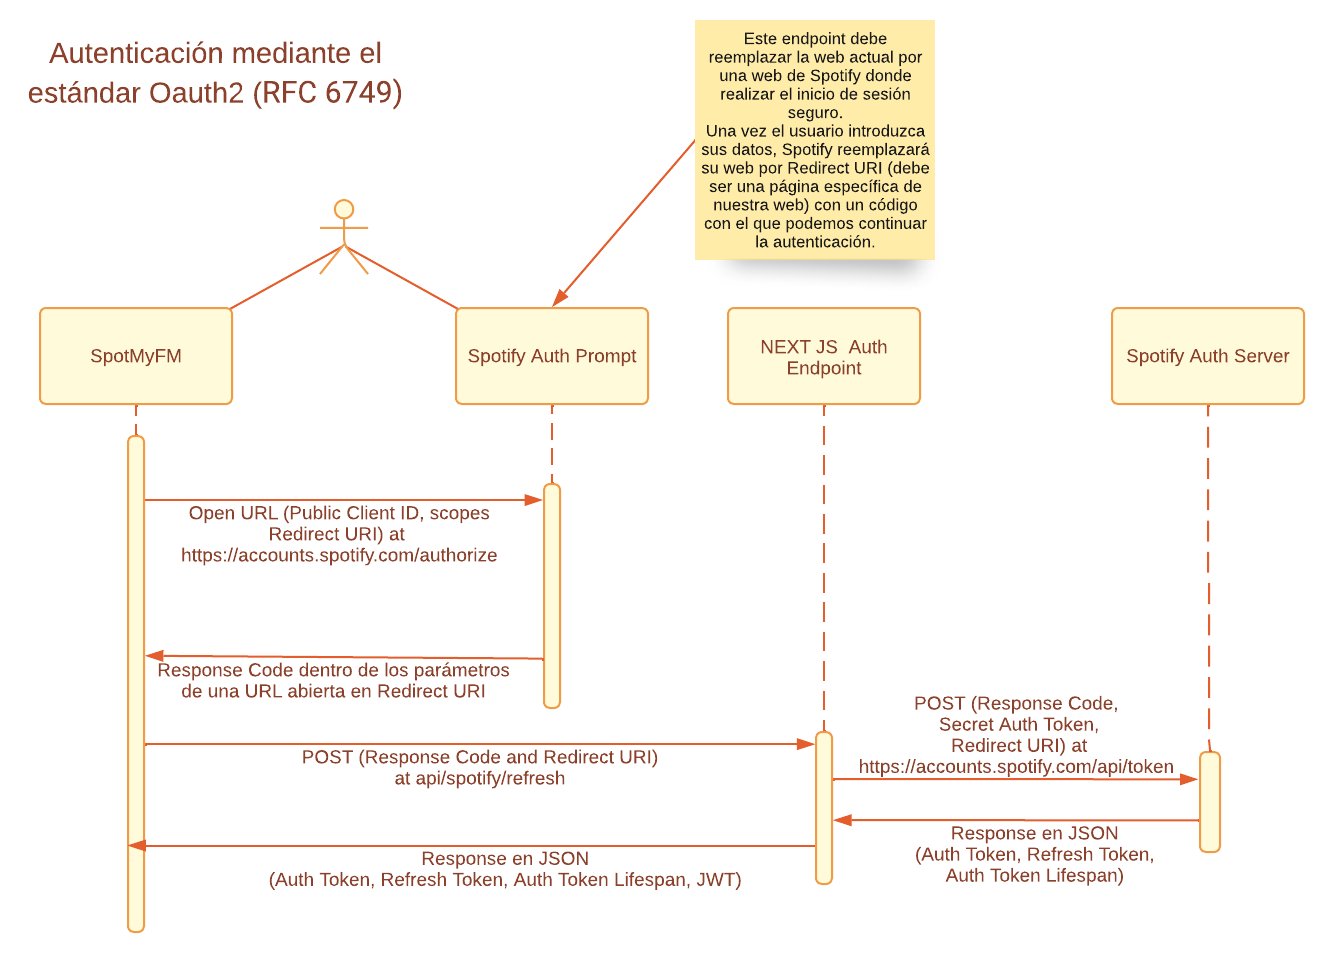
\includegraphics{img/C/oauth2.png}
    \caption{Flujo de Autenticación OAUTH2}
    \label{fig:oauth2_flow}
\end{figure}

En este flujo de autenticación \ref{fig:oauth2_flow}, el usuario abre una URL especial con el token público en los parámetros de la URL. Este token permite a Spotify identificar la aplicación, mostrando al usuario el nombre de la aplicación y los permisos que tiene que otorgar a la aplicación.\footnote{Estos permisos son conocidos en el estándar OAUTH2 como Scopes. }

Si el usuario acepta los permisos, Spotify abrirá una nueva pestaña con un segundo token de verificación en los parámetros de la URL. Este nuevo token se enviará al servidor web, donde se juntará con el token secreto para generar dos nuevos tokenes: un \textbf{token de autenticación} y un \textbf{token de refresco}. El token de autenticación permite al usuario interactuar con la API durante 1h, y el token de refresco permite generar nuevos tokenes de autenticación de 1h para que el usuario no tenga que iniciar sesión cada vez que pase 1h de uso.

En este paso aprovechamos a generar un token JWT con una vida útil de 1h con el siguiente contenido:

\begin{itemize}
    \item Token de Autenticación.
    \item Nombre de usuario.
    \item Identificador interno de Spotify.
    \item Booleano que indica si el usuario está suscrito a Spotify Premium.
\end{itemize}

Hecho estos devolvemos los 3 Tokens al frontend, donde se almacenarán en varias cookies para que sean accesibles entre sesiones. 

Para facilitar la gestión del flujo OAUTH2, se han diseñado dos clases \ref{fig:oauth_class} compatibles con el procedimiento que realizan esta tarea.

\begin{figure}
    \centering
    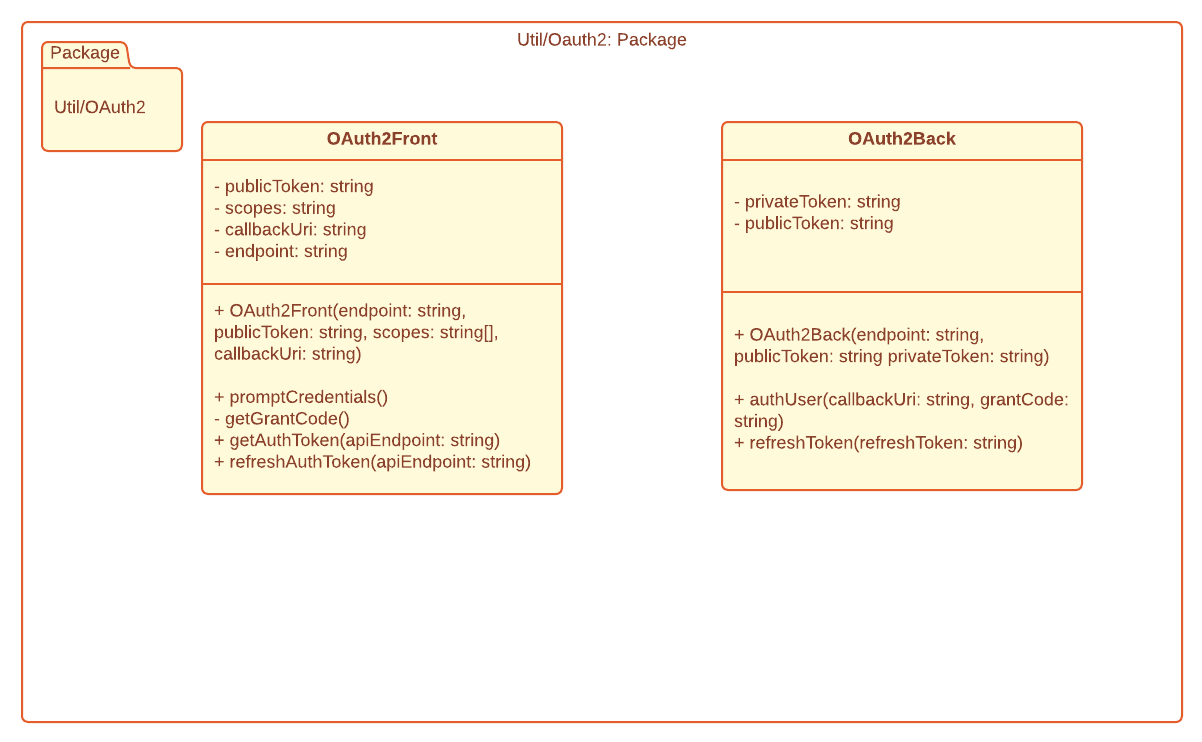
\includegraphics{img/C/oauth2_class_diag.png}
    \caption{Clases auxiliares para el flujo Oauth2}
    \label{fig:oauth_class}
\end{figure}

\subsection{Obtención de los Datos}\label{C:obtencion_datos_flow}

Uno de los objetivos de la fachada de datos \ref{C:fachada_datos} es unificar las distintas fuentes de datos para generar los objetos Fig.\ref{C:datos_front} con los que va a trabajar el presentador. Para ello se han planteado los siguientes diagramas de secuencia, que explican como obtener los datos de forma eficiente de cada una de las fuentes de datos. 

La figura \ref{fig:C:spotify_fetch} hace referencia a como se obtienen todas las canciones completas a partir de una lista de IDs realizando el menor número de peticiones posible. 

\begin{figure}
    \centering
    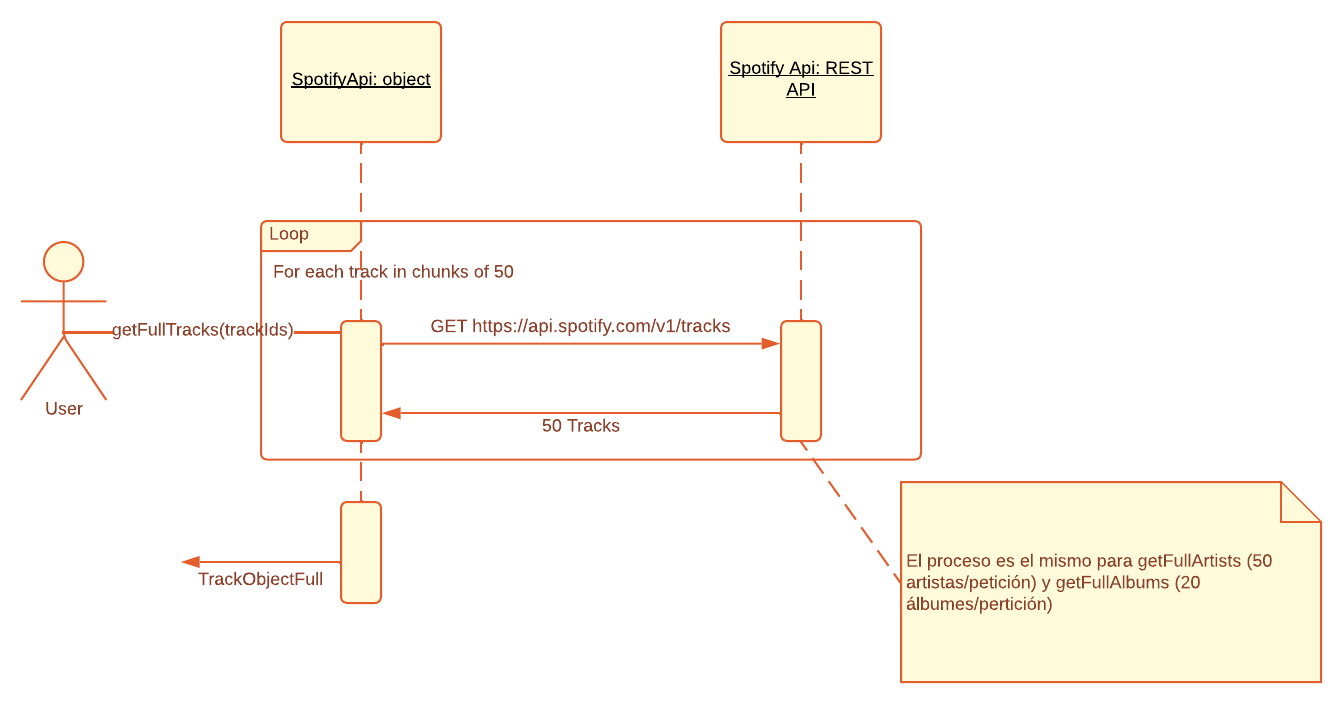
\includegraphics{img/C/spotify_data_fetch.png}
    \caption{Obtención de datos de Spotify}
    \label{fig:C:spotify_fetch}
\end{figure}

La figura \ref{fig:C:ludwig_fetch} explica como se analizan las canciones de Spotify teniendo en cuenta que cada canción analizada se persiste en una base de datos para reducir el tiempo de análisis. 



\begin{figure}
    \centering
    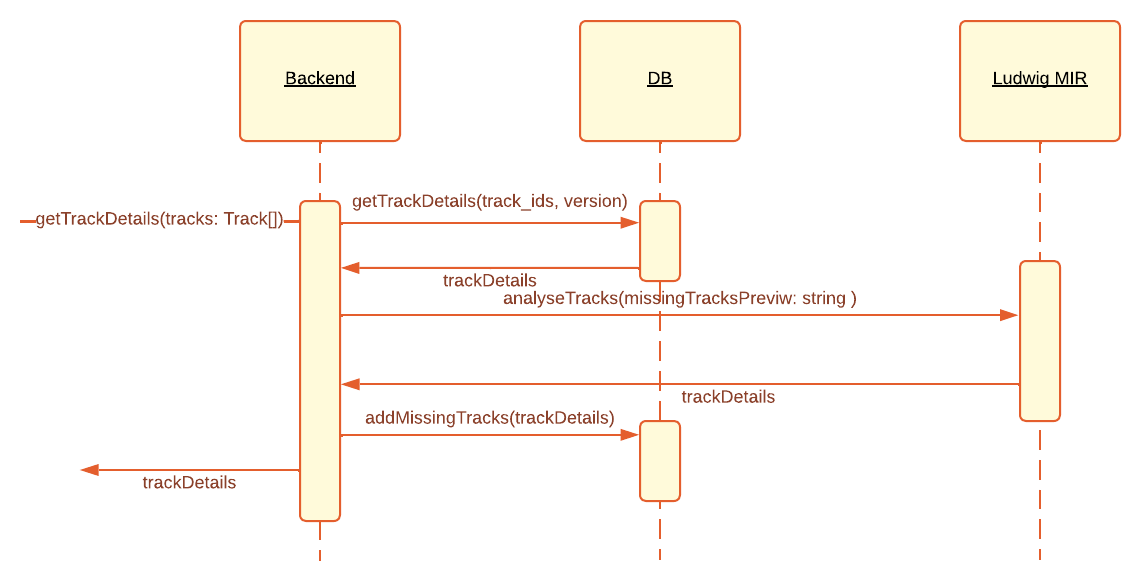
\includegraphics[]{img/C/ludwig_data_fetch.png}
    \caption{Obtención de datos de Ludwig MIR}
    \label{fig:C:ludwig_fetch}
\end{figure}

La figura \ref{fig:C:track_fetch}, al igual que las figuras \ref{fig:C:album_fetch} y \ref{fig:C:artist_fetch} hace referencia a como obtener datos homogéneos a partir de la API de Spotify, LastFM y el Backend Nextjs\footnote{El backend NextJS a su vez se comunica con el Backend de recuperación de información musical y la base de datos}.

La obtención de canciones homogéneas se puede resumir en los siguientes pasos:
    
\begin{enumerate}
    \item  Carga los elementos de la caché a partir de su ID y calcula los elementos que no están cacheados.
    \item Pide a Spotify mediante el proceso de la figura \ref{fig:C:spotify_fetch} las canciones completas. 
    \item Pide al servidor web Ludwig que analice todas las canciones. Este paso se inicia en este punto porque es paso más largo.
    \item Realiza el proceso de la fachada con los artistas Fig.\ref{fig:C:artist_fetch} y álbumes Fig.\ref{fig:C:album_fetch} con todos los álbumes y artistas que ha devuelto la API de Spotify.
    \item Una vez acabados los pasos anteriores, realiza una operación de $join$ que une cada canción con su álbum y artista asociado, esta operación además persiste los datos en la caché local.
    \item Devuelve las canciones homogéneas. Las canciones será actualizadas por referencia una vez se obtengan los resultados del análisis. 
\end{enumerate}


\begin{figure}
    \centering
    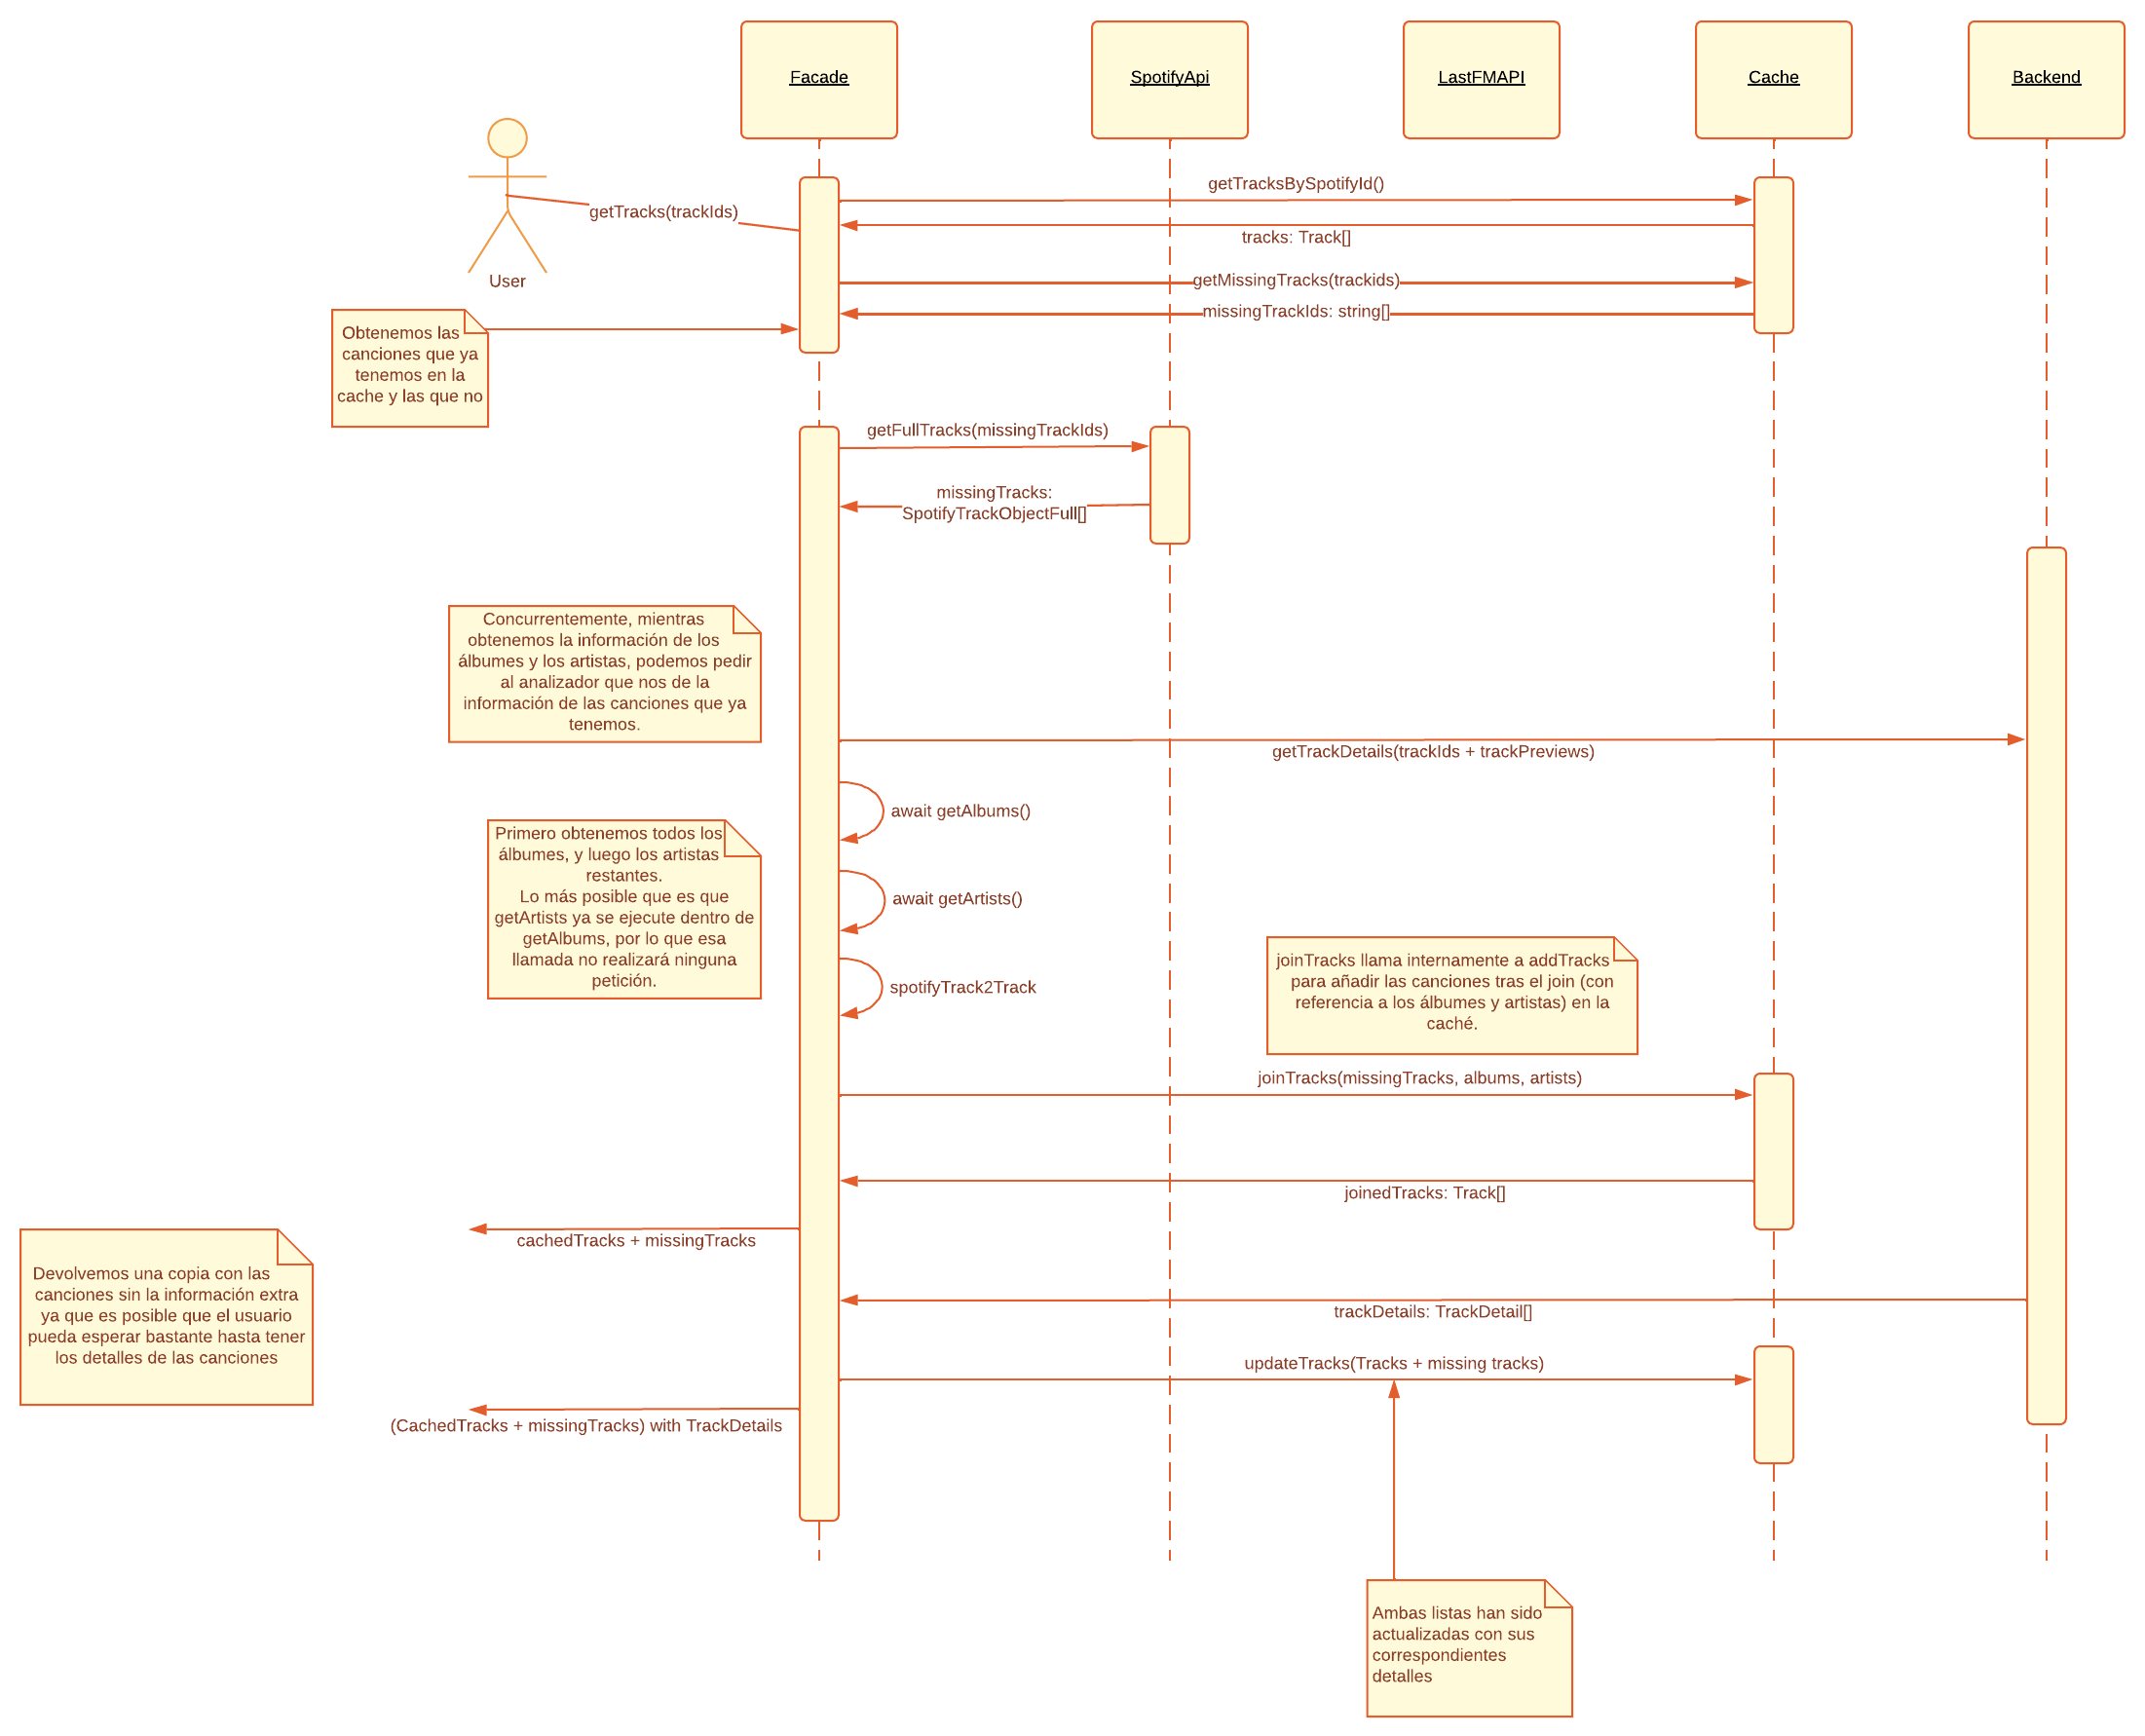
\includegraphics[angle=90]{img/C/track_fetch.png}
    \caption{Obtención de canciones de Spotify}
    \label{fig:C:track_fetch}
\end{figure}


\begin{figure}
    \centering
    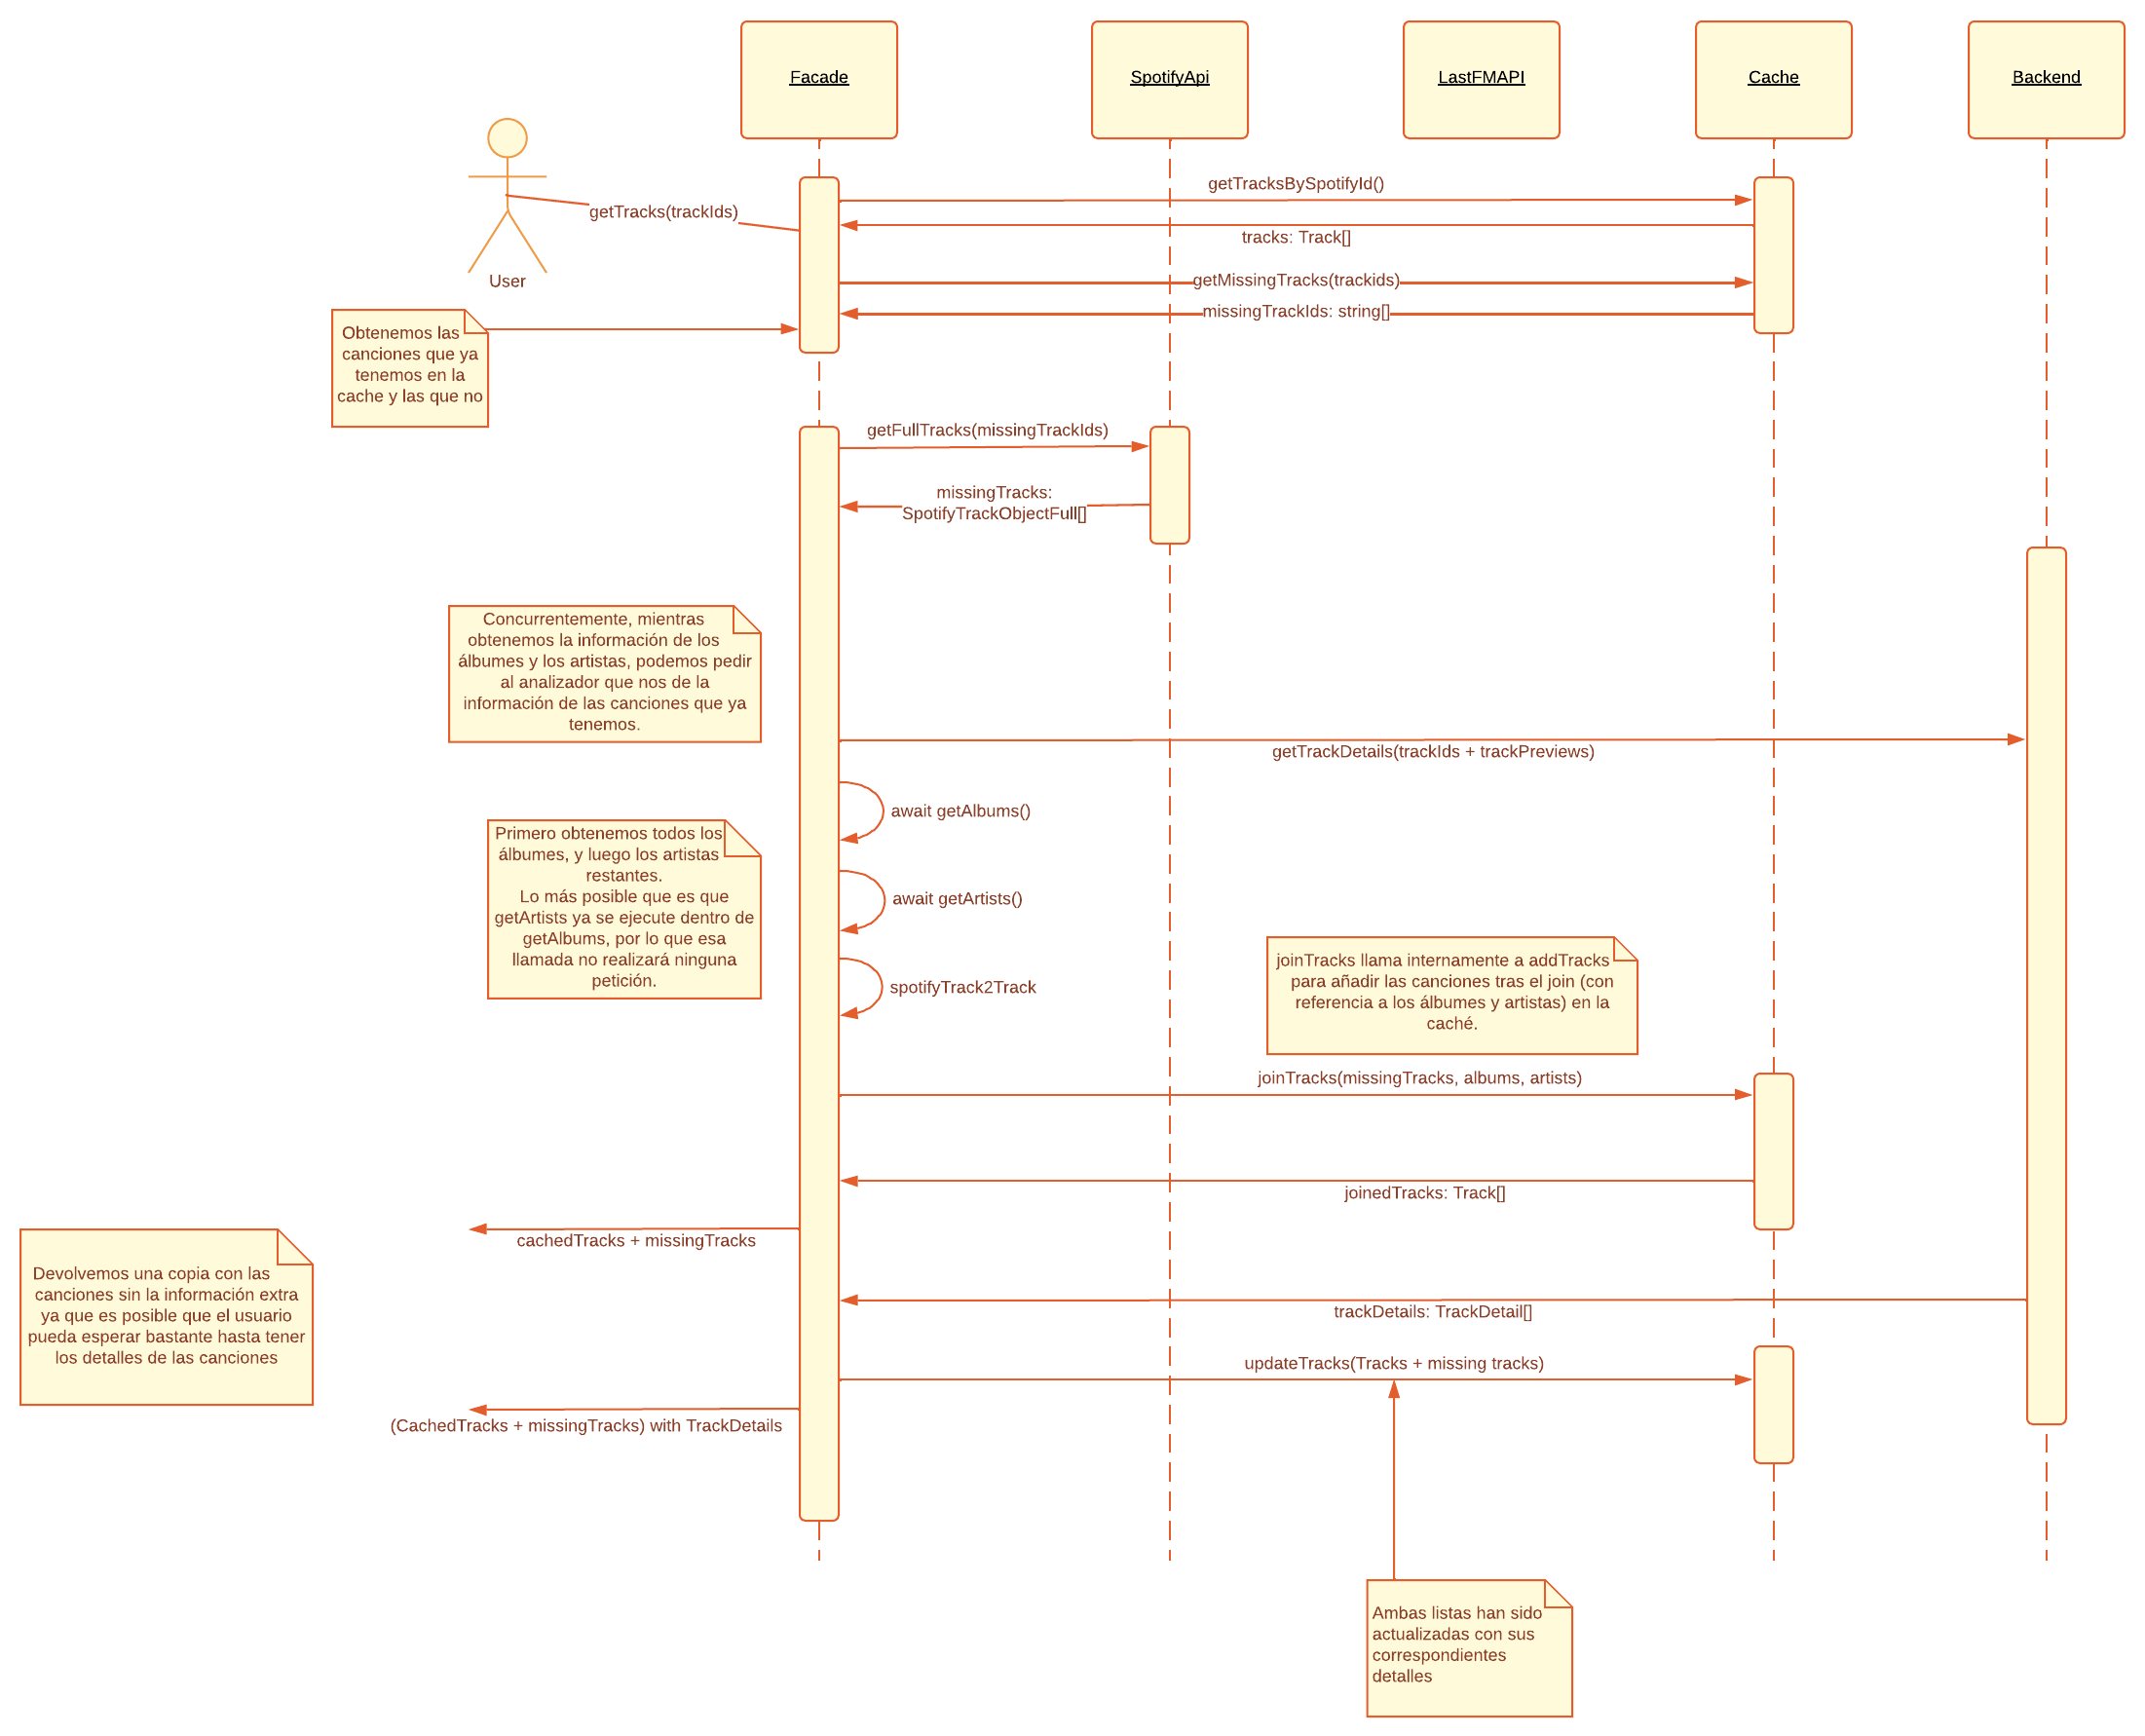
\includegraphics[angle=90]{img/C/track_fetch.png}
    \caption{Obtención de álbumes de Spotify}
    \label{fig:C:album_fetch}
\end{figure}

\begin{figure}
    \centering
    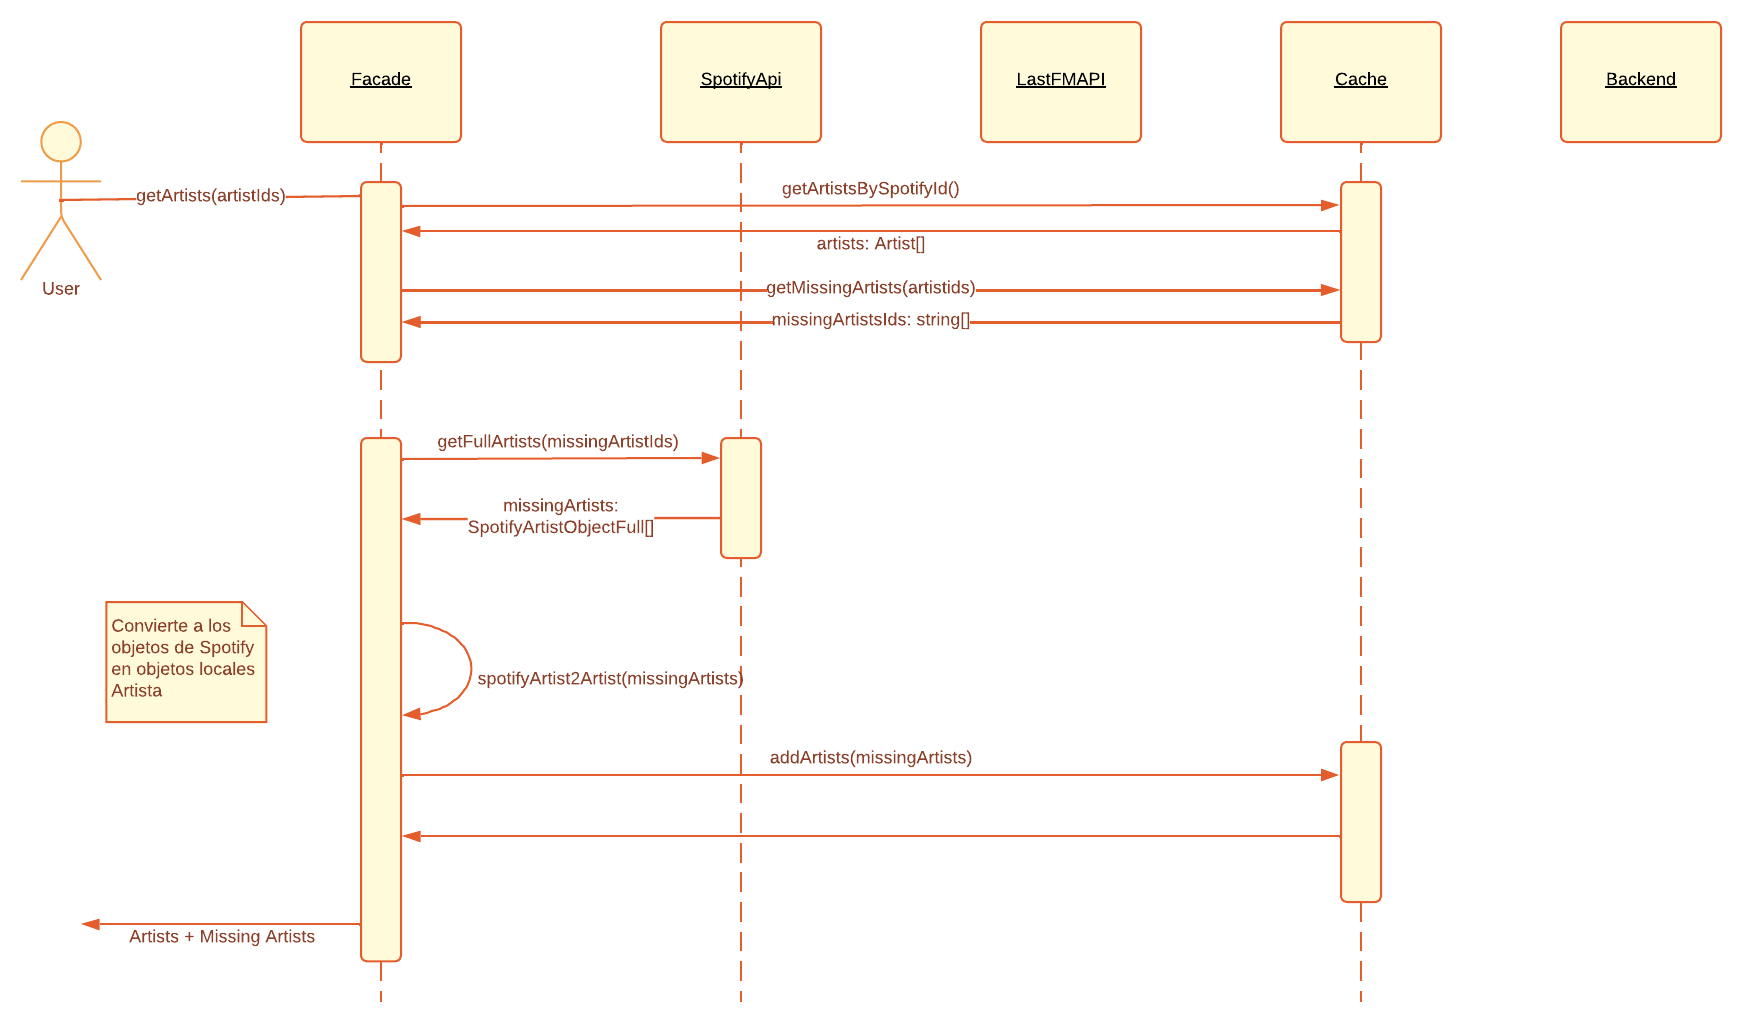
\includegraphics[angle=90]{img/C/artist_fetch.png}
    \caption{Obtención de artistas de Spotify}
    \label{fig:C:artist_fetch}
\end{figure}

\clearpage

\section{Diseño Arquitectónico}

Este apartado concreta los elementos más relevantes sobre la arquitectura del proyecto. 

\subsection{Motor de Inferencia}

Para gestionar el elevado número de clasificadores de subgéneros, se ha diseñado el motor de inferencia recursivo de la figura \ref{fig:C:IE} aplicando el patrón de diseño Composite \cite{C:Composit36:online}. Este motor se configura mediante un fichero .json, donde se recogen los géneros y subgéneros de cada uno de los clasificadores, así como la ruta del modelo en formato ONNX. 

El motor de inferencia agrupa los distintos MFCCs de 3s de duración en un único lote, minimizando el tiempo de inferencia. Cada lote agrupa las $Inference Request$\footnote{Peticiones de Inferencia} por su género o subgénero. Por ejemplo, el clasificador de géneros agrupará las peticiones de inferencia en 9 grupos, siendo cada grupo un género musical. El nodo pasará cada uno de los lotes a su correspondiente Nodo Hijo, que etiquetará los subgéneros de cada canción actualizando el campo de la petición por referencia.


\begin{figure}
    \centering
    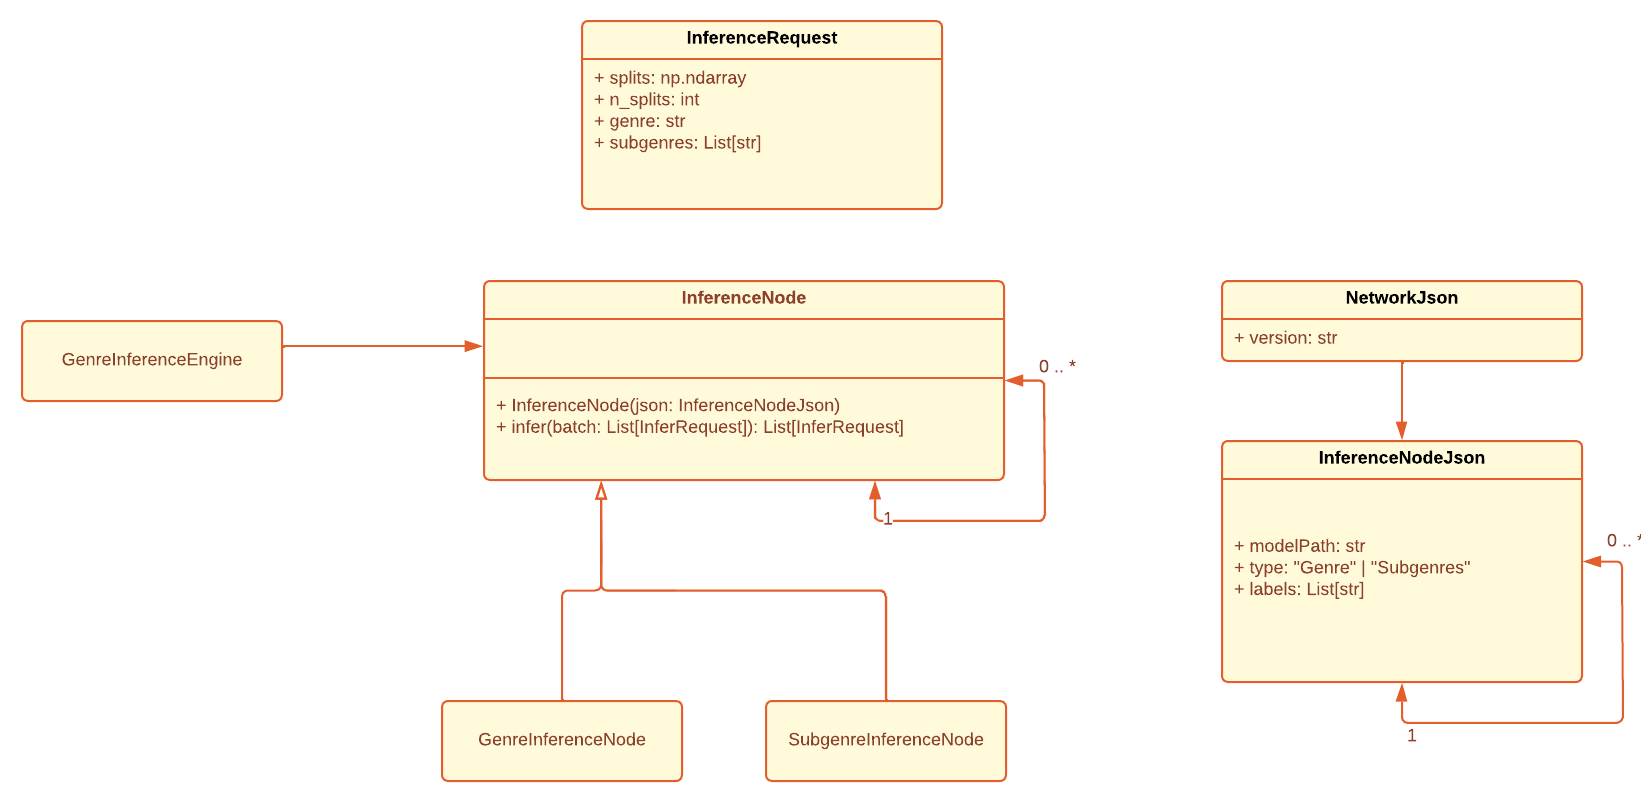
\includegraphics{img/C/IE.png}
    \caption{Motor de Inferencia}
    \label{fig:C:IE}
\end{figure}


\subsection{Patrón MVP} \label{modelo_vista_presentador}

El patrón Modelo Vista Presentador \cite{C:MVP:enwiki:1054194939} es un patrón de software utilizado para construir interfaces.\\
En este patrón nos encontramos tres componentes:
\begin{enumerate}
    \item \textbf{Modelo}: Formado por los datos que va a utilizar el Presentador.
    \item \textbf{Vista}: La interfaz pasiva que muestra los datos procesados por el Presentador.
    \item \textbf{Presentador}: Es el elemento que interactúa entre el Modelo y la Vista, permite obtener los datos de la vista (entrada de usuario) y del modelo, procesarlos y modificar la vista en función a los cambios. 
\end{enumerate}

En este proyecto, el Modelo es la caché de datos y los distintos clientes REST, la vista es el Javascript y HTML generado por ReactJs y el presentador son los Componentes y Hooks de ReactJS escritos en TSX y TS respectivamente. 

\subsection{Fachada de Datos}\label{C:fachada_datos}

Para gestionar el flujo de datos especificado en los diagramas de secuencia  del aparatado \ref{C:obtencion_datos_flow}, se ha detallado un diagrama de clases en la figura \ref{fig:C:facade} con todos los métodos necesarios que detallan las distintas interfaces de los clientes REST, caché local, etc.

En este caso, todos los clientes REST implementan una interfaz común para tratar los errores HTTP, independientemente del cliente HTTP utilizado. 

\begin{figure}
    \centering
    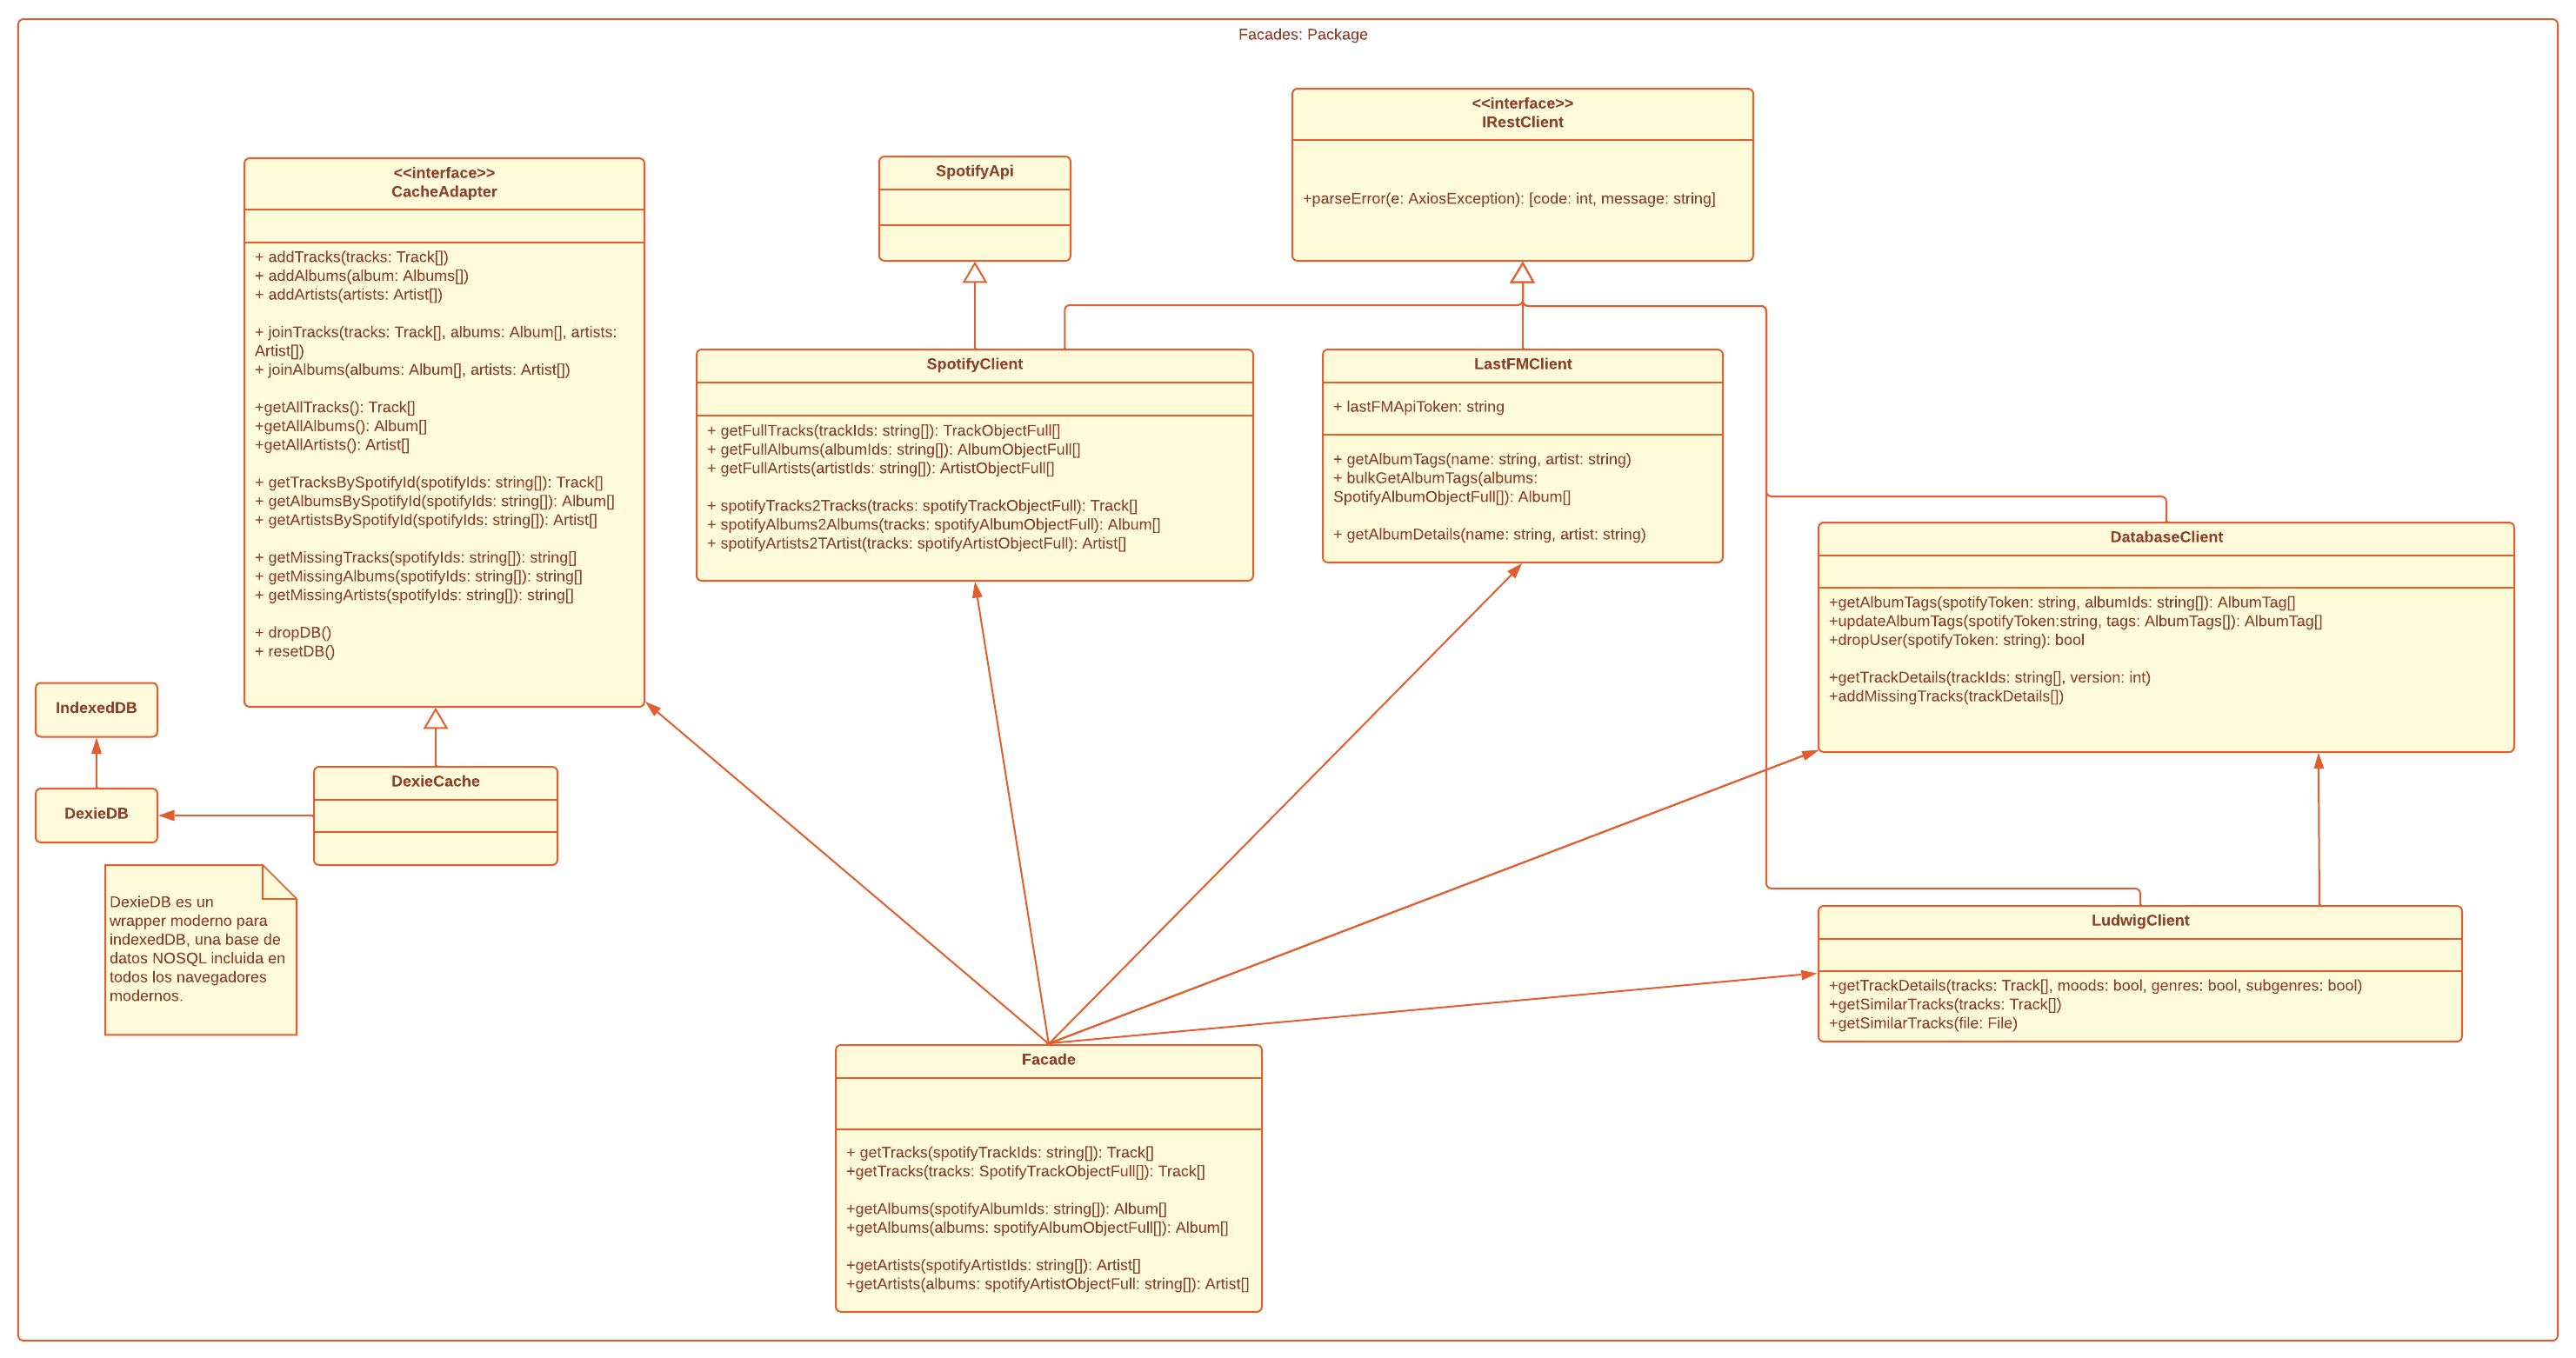
\includegraphics[angle=90,width=\linewidth,height=\textheight,keepaspectratio]{img/C/facade.png}
    \caption{Fachada de Datos}
    \label{fig:C:facade}
\end{figure}


\subsection{Modelo Serverless}

El modelo serverless es un tipo de arquitectura de Cloud Computing que permiten ejecutar y escalar un servicio web sin necesidad de gestionar las máquinas físicas o servidores. 
En el caso de este proyecto, se han usado dos paradigmas serverless: Functions as a Service (FaaS) y Containers as a Service (CaaS). 

Functions as a Service es un paradigma que permite ejecutar funciones sueltas como si fuesen un endpoint de una API. En este caso, por cada petición se levanta un pequeño servicio en los servidores del proveedor cloud, que gestionará la petición HTTP. Una vez se termine la petición, se elimina la instancia de la función.
Podemos disfrutar de este paradigma si desplegamos la platforma con un proveedor cloud compatible, como Netlify o Vercel. 

Containers as a Service es un paradigma que permite instanciar APIs almacenadas en un contenedor de manera similar a FaaS. En este caso, el proveedor cloud permite tener una pool de contenedores, y esta se gestiona automáticamente dependiendo de las necesidades del servicio.
Los dos servidores se han desplegado siguiendo este paradigma. 

Ambos paradigmas permiten escalar de una forma muy directa los distintos servicios, ya que se pueden desplegar tantos servicios como peticiones y en los servidores más cercanos al usuario. El principal inconveniente de estos paradigmas es el tiempo de arranque, ya que si la función o el contenedor tiene un gran número de dependencias, el arranque puede durar varios segundos para gestionar una petición HTTP pequeña que apenas requiere unos pocos cientos de milisegundos de tiempo de ejecución.


\subsection{Guía de Estilo}
Este apartado contiene una guía de estilo con los colores y tamaños de letra utilizados en el frontend. La guía ha sido generada mediante la herramienta Catalog \cite{Catalog1:online}

\label{anexo:guia_estilo}
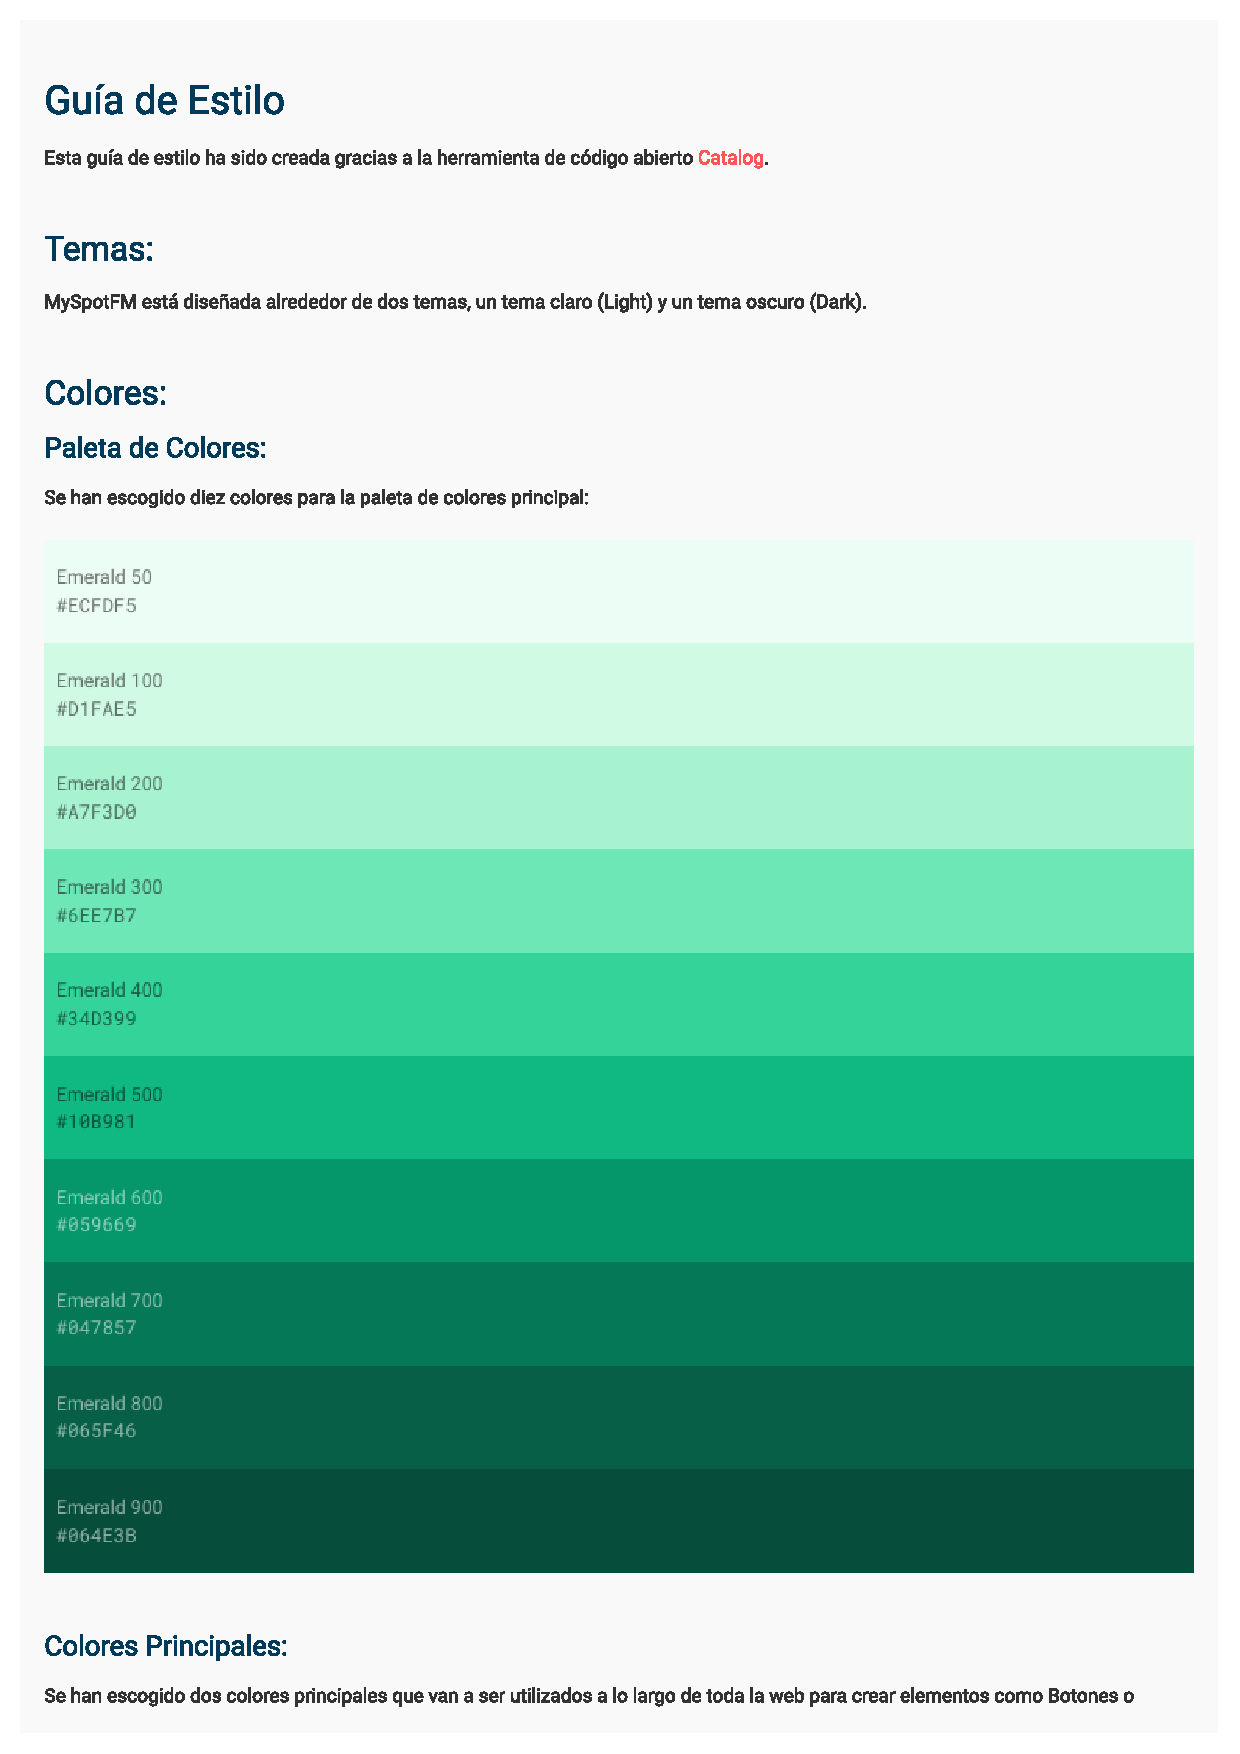
\includepdf[pages=-]{img/C/StyleGuideExport.pdf}
\clearpage
\section{Diseño de Redes Neuronales}

Este apartado detalla la arquitectura de las redes neuronales convolucionales que se han utilizado a lo largo del proyecto. Todas la redes tienen como entrada un tensor con dimensión $N\times130\times32$, correspondiente a un bloque de $N$ MFCCs de 3 segundos de duración.

\subsection{CNN: Clasificador de Géneros}
El clasificador de géneros está formado por 2 redes neuronales. Por un lado se ha utilizado la arquitectura EfficientNetB0 \cite{C:efficentnet} como base del clasificador. Esta arquitectura requiere que la entrada tenga 3 canales, ya que está pensada para el tratamiento de imágenes RGB, por lo que es necesario añadir 2 canales a nuestros MFCCs. Para ello se ha usado una capa convolucional como entrada de la red, que permite expandir la entrada con otras 2 copias.
A la salida de la red EfficientNetB0, se ha añadido una capa GlobalAveragePooling (GAP), que normaliza la salida de la red al realizar una operación de pooling en cada dimensión, reduciendo la dimensión de la salida de forma similar a una capa Flatten. Por último se añaden dos capas densas, la capa de salida con 9 neuronas equivalentes al número de clases, y una capa intermedia entre GAP y la capa de salida, con activación Softmax. Esta red se corresponde con la figura \ref{fig:C:cnn_0}, donde dense\_6 es la salida de la red.

\begin{figure}
    \centering
    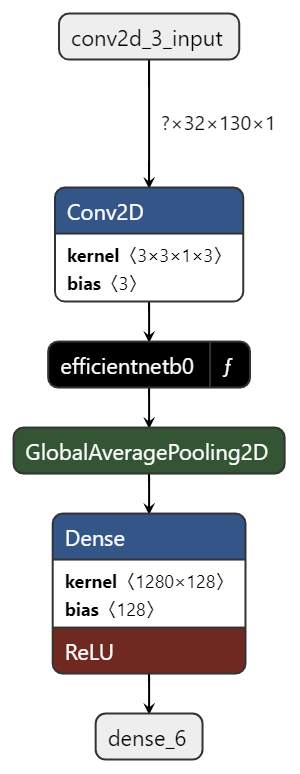
\includegraphics[width=0.33\textwidth,height=\textheight,keepaspectratio]{img/C/cnn_genre_0.png}
    \caption{Arquitectura del Clasificador de Géneros}
    \label{fig:C:cnn_0}
\end{figure}

\subsection{CNN: Clasificador de Subgéneros}\label{c:clas_subg}

El clasificador de subgéneros es una red neuronal convolucional convencional \ref{fig:C:cnn_subgéneros}, formada por bloques convolucionales formados por:

\begin{itemize}
    \item Operación de convolución.
    \item Operación de normalización.
    \item Operación de Pooling.
    \item Segunda operación de normalización.
\end{itemize}

En este caso, la salida de la red es una capa densa con $N$ neuronas, siendo $N$ el número de subgéneros que es capaz de detectar dicha capa. Esta capa tiene como función de activación la función Sigmoide. 

\begin{figure}
    \centering
    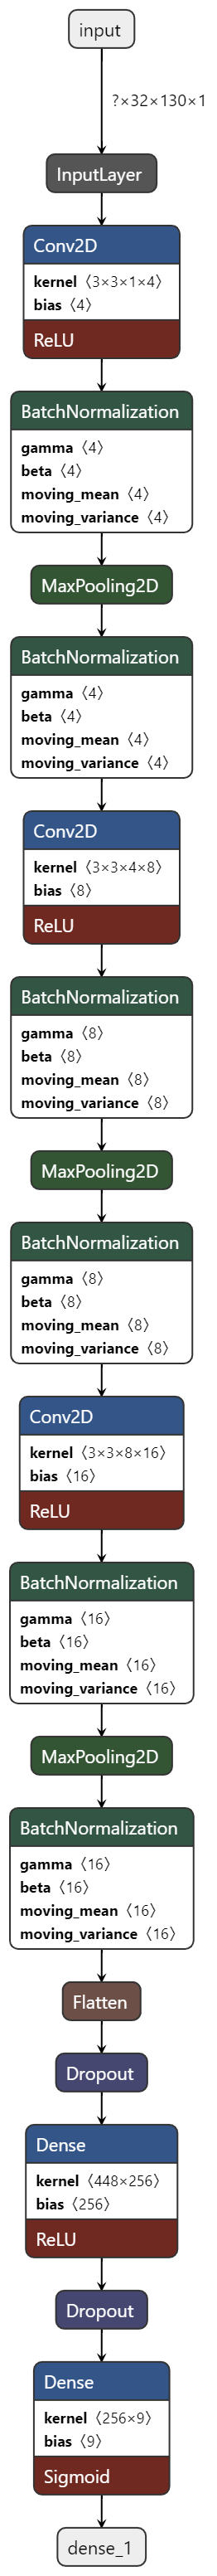
\includegraphics[width=\textwidth,height=\textheight,keepaspectratio]{img/C/cnn_sub.png}
    \caption{Arquitectura del Clasificador de Subgéneros}
    \label{fig:C:cnn_subgéneros}
\end{figure}


\subsection{Ova de CNN: Clasificador de Estados de Ánimo}

El clasificador de estados de ánimo \ref{fig:C:ova} es una OVA de 7 CNNs binarias activadas mediante una Sigmoide. Cada una de las CNNs tiene una arquitectura muy similar a \ref{c:clas_subg}.\\
La salida de la red es una capa de concatenación que junta todas las salidas en un único tensor.

\begin{figure}
    \centering
    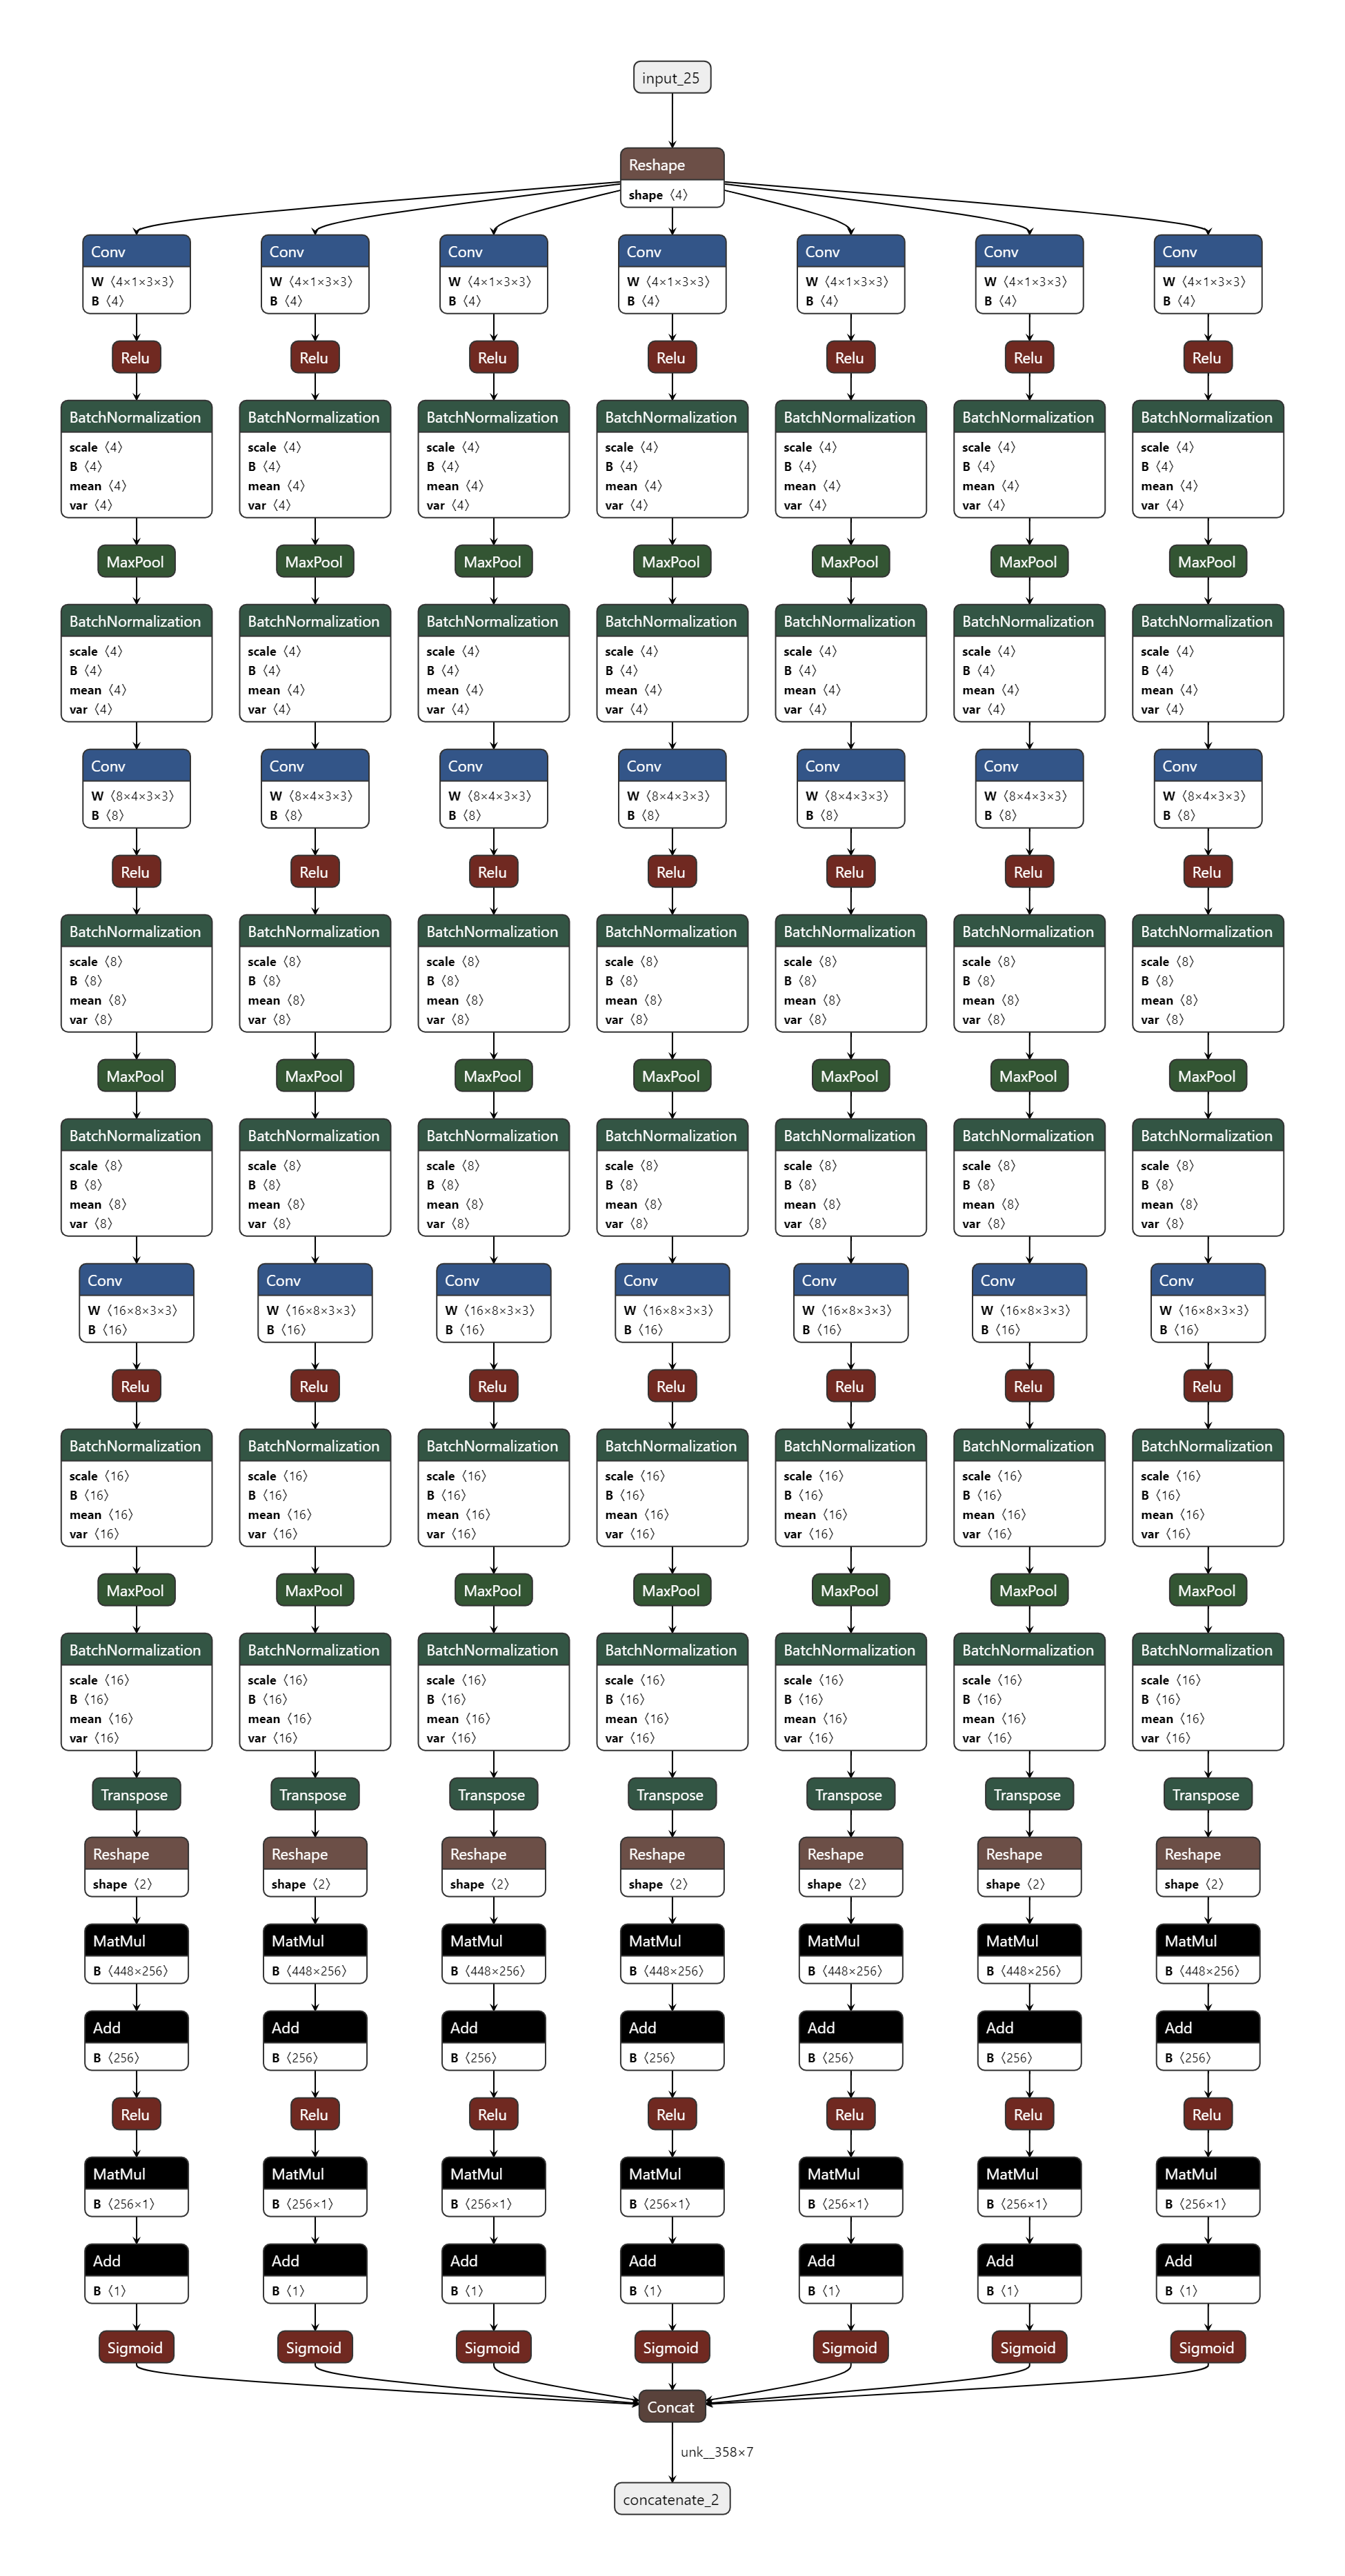
\includegraphics[width=\textwidth,height=\textheight,keepaspectratio]{img/C/cnn_moods_ova.png}
    \caption{Arquitectura del Clasificador de Estados de Ánimo}
    \label{fig:C:ova}
\end{figure}


\apendice{Documentación técnica de programación}

\section{Introducción}

\section{Estructura de directorios}

\section{Manual del programador}

\section{Compilación, instalación y ejecución del proyecto}

\section{Pruebas del sistema}

\apendice{Documentación de usuario}

\section{Introducción}

\section{Requisitos de usuarios}

\section{Instalación}

\section{Manual del usuario}






\bibliographystyle{plain}
\bibliography{bibliografiaAnexos}

\end{document}
